%% The Payne Zero Project II
%% Astronomy & Astrophysics, aa.cls v9.0 (see paper/README.md for provenance).
%%
%% Every number in the text and in the tables is generated by
%% paper/collect_numbers.py from the recorded result artifacts; see
%% Appendix~\ref{app:provenance}.
%% Do not edit numbers or table bodies by hand.
\documentclass{aa}

\usepackage{graphicx}
\usepackage{txfonts}
\usepackage{amsmath}
\usepackage{array}
\usepackage[T1]{fontenc}
\usepackage{hyperref}
\hypersetup{colorlinks=true, allcolors=blue}

\graphicspath{{figs/}}

% Generated by paper/collect_numbers.py -- do not edit by hand.
% Every macro below traces to a result artifact; see paper/numbers.json.

\newcommand{\NOracleElectronDensity}{\ensuremath{5.67\times10^{-4}}}
\newcommand{\NOracleGasPressure}{\ensuremath{4.05\times10^{-4}}}
\newcommand{\NOracleRadiativeAcceleration}{\ensuremath{8.47\times10^{-4}}}
\newcommand{\NOracleRosselandOpacity}{\ensuremath{8.74\times10^{-4}}}
\newcommand{\NSixfieldElectronDensity}{\ensuremath{1.30\times10^{-2}}}
\newcommand{\NSixfieldGasPressure}{\ensuremath{1.81\times10^{-2}}}
\newcommand{\NSixfieldRadiativeAcceleration}{\ensuremath{3.18\times10^{-2}}}
\newcommand{\NSixfieldRosselandOpacity}{\ensuremath{1.43\times10^{-2}}}
\newcommand{\NTwofieldElectronDensity}{\ensuremath{5.24\times10^{-3}}}
\newcommand{\NTwofieldGasPressure}{\ensuremath{4.51\times10^{-3}}}
\newcommand{\NTwofieldRadiativeAcceleration}{\ensuremath{5.59\times10^{-3}}}
\newcommand{\NTwofieldRosselandOpacity}{\ensuremath{5.21\times10^{-3}}}
\newcommand{\NanalyticCommon}{56}
\newcommand{\NanalyticCompression}{361}
\newcommand{\NanalyticConstants}{2\,407}
\newcommand{\NanalyticConverged}{57}
\newcommand{\NanalyticFailures}{3}
\newcommand{\NanalyticFaster}{2}
\newcommand{\NanalyticIntegerEntries}{564}
\newcommand{\NanalyticIterDifference}{3.70}
\newcommand{\NanalyticIterMean}{7.77}
\newcommand{\NanalyticIterMedian}{8.0}
\newcommand{\NanalyticIterationLimit}{15}
\newcommand{\NanalyticLearnedFaster}{54}
\newcommand{\NanalyticLearnedOnly}{0}
\newcommand{\NanalyticMassPenalty}{5.8}
\newcommand{\NanalyticMassPfive}{\ensuremath{8.76\times10^{-2}}}
\newcommand{\NanalyticOnly}{1}
\newcommand{\NanalyticSerializedFloats}{2\,417}
\newcommand{\NanalyticTempPenalty}{5.1}
\newcommand{\NanalyticTempPfive}{\ensuremath{1.91\times10^{-2}}}
\newcommand{\NanalyticTied}{0}
\newcommand{\NanalyticTimeoutSeconds}{900}
\newcommand{\NanalyticTimeouts}{0}
\newcommand{\NanalyticTrainStars}{40\,911}
\newcommand{\NanalyticValStars}{10\,228}
\newcommand{\NblindCandIters}{4.12}
\newcommand{\NblindCandNonmono}{26.8\%}
\newcommand{\NblindCandUsable}{190}
\newcommand{\NblindFaster}{138}
\newcommand{\NblindMassBlowouts}{18}
\newcommand{\NblindMassLimit}{\ensuremath{1.52\times10^{-2}}}
\newcommand{\NblindMassPfive}{\ensuremath{2.66\times10^{-2}}}
\newcommand{\NblindMcnemarP}{\ensuremath{1.6\times10^{-21}}}
\newcommand{\NblindPaired}{188}
\newcommand{\NblindPairedDiffCiHi}{1.87}
\newcommand{\NblindPairedDiffCiLo}{1.28}
\newcommand{\NblindPairedDiffMean}{1.57}
\newcommand{\NblindPairedDiffMedian}{1.50}
\newcommand{\NblindProdIters}{5.69}
\newcommand{\NblindProdNonmono}{53.0\%}
\newcommand{\NblindProdUsable}{193}
\newcommand{\NblindSame}{32}
\newcommand{\NblindSelectionSeed}{20260811}
\newcommand{\NblindSlower}{18}
\newcommand{\NblindSpecMax}{\ensuremath{1.42\times10^{-2}}}
\newcommand{\NblindSpecMedian}{\ensuremath{2.03\times10^{-3}}}
\newcommand{\NblindSpecOver}{25}
\newcommand{\NblindStars}{200}
\newcommand{\NblindTempBlowouts}{6}
\newcommand{\NblindTempLimit}{\ensuremath{3.74\times10^{-3}}}
\newcommand{\NblindTempPfive}{\ensuremath{3.38\times10^{-3}}}
\newcommand{\NblindUnionBlowouts}{19}
\newcommand{\NboxConverged}{85.3\%}
\newcommand{\NboxFailed}{14.7\%}
\newcommand{\NboxNonmono}{64\%}
\newcommand{\NboxQ}{0.752}
\newcommand{\NboxRecoverable}{69.8\%}
\newcommand{\NbrokenCount}{325}
\newcommand{\NbrokenIters}{19}
\newcommand{\NbrokenLogg}{2.54}
\newcommand{\NbrokenMetal}{-1.16}
\newcommand{\NcorpusStars}{52\,199}
\newcommand{\NderivedLearnedFailures}{1}
\newcommand{\NderivedLearnedStars}{59}
\newcommand{\NdevIterMean}{3.77}
\newcommand{\NdevMassPfive}{\ensuremath{1.19\times10^{-2}}}
\newcommand{\NdevQualIters}{3.77}
\newcommand{\NdevSelectionSeed}{20260812}
\newcommand{\NdevSpecOver}{0}
\newcommand{\NdevSpecStars}{60}
\newcommand{\NdevSpecUpper}{4.9\%}
\newcommand{\NdevTempPfive}{\ensuremath{2.06\times10^{-3}}}
\newcommand{\NdirectTempPfive}{\ensuremath{3.22\times10^{-3}}}
\newcommand{\NdirectViolations}{3}
\newcommand{\NevalStars}{60}
\newcommand{\NfieldGainHigh}{5.7}
\newcommand{\NfieldGainLow}{2.5}
\newcommand{\NgateBar}{\ensuremath{5.0\times10^{-3}}}
\newcommand{\NgateResolution}{20\,000}
\newcommand{\NgateWindowHi}{900}
\newcommand{\NgateWindowLo}{400}
\newcommand{\NgridLayers}{80}
\newcommand{\NhardFraction}{33\%}
\newcommand{\NiidConverged}{99.2\%}
\newcommand{\NiidPninety}{8}
\newcommand{\NiterReduction}{28\%}
\newcommand{\NjitterConverged}{93.3\%}
\newcommand{\NjitterGateMax}{\ensuremath{1.50\times10^{-2}}}
\newcommand{\NjitterGateMedian}{\ensuremath{3.44\times10^{-3}}}
\newcommand{\NjitterGateOver}{16}
\newcommand{\NjitterGateStars}{56}
\newcommand{\NjitterIterMean}{7.45}
\newcommand{\NlearnedConverged}{56}
\newcommand{\NlearnedFailures}{4}
\newcommand{\NlearnedFirstResidual}{\ensuremath{2.75\times10^{-3}}}
\newcommand{\NlearnedGainP}{0.002}
\newcommand{\NlearnedGainRho}{0.41}
\newcommand{\NlearnedGateMax}{\ensuremath{5.04\times10^{-3}}}
\newcommand{\NlearnedGateMedian}{\ensuremath{1.61\times10^{-3}}}
\newcommand{\NlearnedGateOver}{1}
\newcommand{\NlearnedGateStars}{56}
\newcommand{\NlearnedHotGain}{2.4}
\newcommand{\NlearnedIterMean}{4.05}
\newcommand{\NlearnedMassPfive}{\ensuremath{1.52\times10^{-2}}}
\newcommand{\NlearnedNonmono}{18.6\%}
\newcommand{\NlearnedQ}{0.547}
\newcommand{\NlearnedReconstructionFailures}{1}
\newcommand{\NlearnedRestGain}{0.7}
\newcommand{\NlearnedRuntimeFloats}{873\,450}
\newcommand{\NlearnedSolverFailures}{3}
\newcommand{\NlearnedTempPfive}{\ensuremath{3.74\times10^{-3}}}
\newcommand{\NmonoTempPfive}{\ensuremath{3.74\times10^{-3}}}
\newcommand{\NmonoViolations}{0}
\newcommand{\NnetDepth}{4}
\newcommand{\NnetEpochs}{300}
\newcommand{\NnetWidth}{512}
\newcommand{\NoracleAtFloor}{55}
\newcommand{\NoracleFirstResidual}{\ensuremath{4.20\times10^{-4}}}
\newcommand{\NoracleGap}{11}
\newcommand{\NoracleGapMax}{2}
\newcommand{\NoracleGapStars}{5}
\newcommand{\NoracleIterMean}{3.37}
\newcommand{\NoracleReconElectronDensity}{\ensuremath{5.67\times10^{-4}}}
\newcommand{\NoracleReconGasPressure}{\ensuremath{4.05\times10^{-4}}}
\newcommand{\NoracleReconRadiativeAcceleration}{\ensuremath{8.47\times10^{-4}}}
\newcommand{\NoracleReconRosselandOpacity}{\ensuremath{8.74\times10^{-4}}}
\newcommand{\NprodFailures}{1}
\newcommand{\NprodFirstResidual}{\ensuremath{2.44\times10^{-3}}}
\newcommand{\NprodIterMean}{5.59}
\newcommand{\NprodMassPfive}{\ensuremath{2.39\times10^{-2}}}
\newcommand{\NprodNonmono}{53.3\%}
\newcommand{\NprodQ}{0.656}
\newcommand{\NprodTempPfive}{\ensuremath{4.02\times10^{-3}}}
\newcommand{\NredGiantOneSided}{96.1\%}
\newcommand{\NresCoarse}{40}
\newcommand{\NresCoarseError}{\ensuremath{3.08\times10^{-5}}}
\newcommand{\NresFinest}{640}
\newcommand{\NresFinestError}{\ensuremath{6.55\times10^{-9}}}
\newcommand{\NrestIters}{10}
\newcommand{\NrestLogg}{3.28}
\newcommand{\NrestMetal}{-1.02}
\newcommand{\NseedAboveHundredth}{8.33\%}
\newcommand{\NseedAboveTenth}{0.62\%}
\newcommand{\NseedMax}{1.689}
\newcommand{\NseedMedian}{\ensuremath{7.37\times10^{-4}}}
\newcommand{\NseedPninetynine}{0.0739}
\newcommand{\NseedSpearman}{-0.043}
\newcommand{\NsixAtFloor}{57}
\newcommand{\NsixIterMean}{3.23}
\newcommand{\NsyncMaxPasses}{8}
\newcommand{\NsyncPasses}{3}
\newcommand{\NsyncPressureTolerance}{\ensuremath{1.00\times10^{-3}}}
\newcommand{\NtrainSeed}{20260807}
\newcommand{\NtrainStars}{41\,867}
\newcommand{\NtruthGateFactor}{60}
\newcommand{\NtruthGateMax}{\ensuremath{1.39\times10^{-3}}}
\newcommand{\NtruthGateMedian}{\ensuremath{8.28\times10^{-5}}}
\newcommand{\NtruthGateOver}{0}
\newcommand{\NtruthGateStars}{60}
\newcommand{\NvalStars}{10\,272}


\begin{document}

% TODO: confirm affiliations before submission (both authors share the MPIA
% address below; Ting's second affiliation is TBD).
\title{A Solver-Consistent Two-Field Representation for 1D LTE Model-Atmosphere Initialization}

\author{Jiadong Li\inst{1}, Yuan-Sen Ting\inst{1,2}}

\institute{Max Planck Institute for Astronomy\\
  \email{jdli@mpia.de}}


\date{Received ---; accepted ---}

\abstract
{A stellar atmosphere is commonly stored as a set of depth-dependent fields,
yet those fields are not independent: the equation of state, hydrostatic
balance, opacity and radiative transfer couple them tightly. We investigate
whether this physical structure admits a reduced description in terms of two
depth-dependent coordinates alone, column mass and temperature, with the
remaining fields reconstructed by the atmosphere solver itself. Framing the
problem in this way separates the dimensionality of the physical state from
the accuracy of any model trained to predict it. At the representation level,
the converged two-coordinate state attains the same structural and spectral
fidelity as the released six-field state. A learned predictor of the two
coordinates, rematerialized from labels and hydrostatic balance without
querying the six-field emulator at inference, reduces solver iterations and
oscillations on development data, and this speed advantage survives a sealed
holdout, whereas the profile and spectral reliability of the predictor do
not. Within the tested label range,
the two-coordinate representation is therefore physically sufficient, while
the learned initializer has not yet reached the reliability required to
replace the production model. These findings indicate that further
improvements should target the solver's physical basin of attraction rather
than an increase in the number of independently predicted fields.}

\keywords{stars: atmospheres --
  methods: numerical --
  radiative transfer --
  techniques: spectroscopic --
  stars: fundamental parameters}

\maketitle

%%%%%%%%%%%%%%%%%%%%%%%%%%%%%%%%%%%%%%%%%%%%%%%%%%%%%%%%%%%%%%%%%%%%%%%%%%%%%
\section{Introduction}
\label{sec:intro}

Most abundance measurements from survey spectra rest on a precomputed grid of
model atmospheres, whether ATLAS \citep{kurucz1970, castelli2003}, MARCS
\citep{gustafsson2008} or PHOENIX \citep{hauschildt1999, husser2013},
because computing a dedicated atmosphere for every star has historically been
too expensive for routine analysis. The errors introduced by interpolating
within such grids have been characterized for decades
\citep{meszaros2013}. Payne Zero \citep[hereafter Paper~I]{ting2026} removed
much of this cost by reorganizing the Kurucz calculation so that spectral
synthesis runs on a GPU while the atmosphere iteration runs on multicore
CPUs, reducing the time for a converged atmosphere to a few seconds and
making direct physical fitting of survey spectra practical.

Once the atmosphere solve takes seconds rather than hours, its cost is set by
the number of iterations required to converge, and therefore by the state
from which the iteration starts. Paper~I supplies a learned initializer for
this purpose, a neural network that maps stellar labels to a starting
atmosphere from which the solver then iterates, and at the same time
identifies initialization as the least satisfactory part of the method. The
present paper takes up that problem from a different direction. Rather than
enlarging the network or its training set, we first ask which quantities the
network needs to predict at all.

A converged Payne Zero atmosphere is stored as six fields on each of
\NgridLayers\ depth points: column mass $m$, temperature $T$, gas pressure
$P_{\rm gas}$, electron density $n_{\rm e}$, Rosseland mean opacity
$\kappa_{\rm R}$ and radiative acceleration $g_{\rm rad}$. A learned
initializer that predicts all six therefore reproduces quantities that the
physics already ties together: given the depth coordinate, the composition
and the two thermodynamic profiles, the equation of state fixes the electron
density, the opacity tables fix $\kappa_{\rm R}$, and the transfer solution
fixes $g_{\rm rad}$. Nothing in the training procedure forces a six-output
network to respect those relations. Each field is compared with its own
target, so the network can fit all six well and still return an electron
density that the equation of state would not produce for the temperature and
column mass returned alongside it. Such a state is not simply an inaccurate
atmosphere: because in general no single pair of profiles $(m,T)$ yields the
six predicted fields jointly, it corresponds to no atmosphere that the
solver's own physics could produce. The solver nevertheless iterates on a
state whose fields are tied to one another, and how it behaves when they are
not is the subject of Sect.~\ref{sec:consistency}.

We therefore retain only the two coordinates $m(\tau)$ and $T(\tau)$ and
rebuild the other four fields by running the solver's own equation of state,
opacity, transfer and hydrostatic closure on the unchanged production grid.
Whether this succeeds is decided not by the choice of coordinates but by the
internal consistency of the rebuilt state. A single pass through that chain
leaves the four derived fields mutually inconsistent, and the solver's
ordinary iteration then carries the atmosphere away from the branch that its
coordinates specify. We instead iterate the chain to self-consistency,
holding $m$ and $T$ fixed throughout and reading the derived fields out
before any temperature correction is applied. Rebuilt in this way, the
reduced state proves sufficient at every level at which we are able to test
it.

Several lines of related work approach this construction without coinciding
with it. Interpolation of precomputed atmosphere grids is the classical way
to avoid the cost of a solve, and its error budget in spectra and structure
is well characterized \citep{meszaros2013}; more recently, neural
interpolation of complete atmosphere structures between grid points reaches
high accuracy in the grid's interior \citep[][iNNterpol]{westendorp2023},
and spectral-level neural emulation of the mapping from labels to spectra
underlies The Payne \citep{ting2019}, on which the fitting side of Paper~I
builds. Physics-constrained neural surrogates of the atmosphere structure
itself, with the governing equations entering the loss, have also been
demonstrated \citep[][Kurucz-a1, an arXiv preprint and workshop
paper]{li2025kurucza1}. All of these approaches replace or sidestep the
solver, whereas here the prediction is used only to start the original solver
and acceptance is measured by what the solver itself does with it.

The paper addresses three questions, each supported by a different strength
of evidence. The first is a representation question: are two of the six
stored fields sufficient to rebuild the other four, with no predictor
involved at all? The second is a learning question: can a network predict
those two coordinates well enough to provide a useful warm start? The third
is a generalization question: does a frozen policy built in this way survive
a sealed holdout? The answers are affirmative, affirmative and negative,
respectively, and we report them separately because each rests on a different
experiment.

The remainder of the paper is organized as follows. Section~\ref{sec:solver}
gives the minimal solver description needed to define the reduced state, and
Sect.~\ref{sec:reduced} defines the rematerialization path.
Section~\ref{sec:data} describes the evaluation design.
Section~\ref{sec:results} tests representation sufficiency, compares the
learned two-field initializer with the released baseline, and reports the
sealed holdout. Detailed solver diagnostics, the analytic initializer and
provenance records are collected in the appendices.

%%%%%%%%%%%%%%%%%%%%%%%%%%%%%%%%%%%%%%%%%%%%%%%%%%%%%%%%%%%%%%%%%%%%%%%%%%%%%
\section{The solver and its state}
\label{sec:solver}

\subsection{The carried state and its closure}
\label{sec:state}

The production solver computes a plane-parallel, hydrostatic, one-dimensional
LTE atmosphere on a fixed Rosseland optical-depth grid,
\begin{equation}
  \tau_{\rm std}(i) = 10^{-6.875 + 0.125\,i}, \qquad
  i=0,\ldots,\NgridLayers-1 .
  \label{eq:grid}
\end{equation}
It stores six depth-dependent profiles,
\begin{equation}
  \mathbf{p} =
  \bigl\{m_j,T_j,P_{{\rm gas},j},n_{{\rm e},j},
  \kappa_{{\rm R},j},g_{{\rm rad},j}\bigr\}_{j=1}^{\NgridLayers},
  \label{eq:state}
\end{equation}
namely column mass, temperature, gas pressure, electron density, Rosseland
mean opacity and radiative acceleration. The solver also carries iteration
variables and opacity information that are not part of this physical
projection; the distinction matters because initialization acts on the
complete state.

The closure couples these fields through the equation of state, opacity and
radiative transfer. In particular,
\begin{align}
  g_{\rm rad}(m) &= \frac{1}{c}\int_0^\infty \chi_\nu F_\nu\,{\rm d}\nu,
  \qquad
  P_{\rm rad}(m) = \int_0^m g_{\rm rad}(m')\,{\rm d}m', \label{eq:grad}\\
  P_{\rm gas} &= g\,m-P_{\rm rad}. \label{eq:hse}
\end{align}
Here $\chi_\nu$ is the total extinction per unit mass and $F_\nu$ is the
monochromatic flux. The production branch disables turbulent pressure; the
microturbulent velocity remains a spectral-broadening parameter. At fixed
labels and fixed $(m,T)$, the equation of state, opacity and transfer routines
therefore determine the other four stored fields. This physical closure is the
reason a six-field initializer can contain mutually inconsistent quantities.

\subsection{Energy balance and the temperature correction}
\label{sec:correction}

The ordinary solver does more than synchronize the closure: it changes $T$ and
$m$ until the total flux is constant,
\begin{equation}
  F_{\rm rad}(m)+F_{\rm conv}(m)=\sigma T_{\rm eff}^{4},
  \qquad
  \epsilon_F =
  \frac{F_{\rm rad}+F_{\rm conv}}{\sigma T_{\rm eff}^{4}}-1 .
  \label{eq:energy}
\end{equation}
The production temperature corrections and damping rules are unchanged from
Paper~I and are not modified here. What matters for the present argument is
that a temperature correction also remaps the column-mass coordinate, so that
an internally inconsistent state can drift away from the coordinates supplied
at the handoff.

\subsection{The iteration as a map}
\label{sec:map}

Writing $\mathbf{x}$ for the complete carried state, one production pass can be
summarized as
\begin{equation}
  \begin{aligned}
  \mathbf{x}^{(n)}
  &\longrightarrow
  \bigl(P_{\rm gas},n_{\rm e},\chi_\nu\bigr)^{(n)}
  \longrightarrow
  \bigl(g_{\rm rad},\kappa_{\rm R},F_{\rm conv}\bigr)^{(n)} \\
  &\longrightarrow
  (T,m)^{(n+1)}
  \xrightarrow{\rm remap}
  \mathbf{x}^{(n+1)} ,
  \end{aligned}
  \label{eq:pass}
\end{equation}
or $\mathbf{x}^{(n+1)}=\mathcal{G}(\mathbf{x}^{(n)})$. The converged atmosphere
is the fixed point of this map. Convergence is declared from the deep-layer
temperature change,
\begin{equation}
  \epsilon_T =
  \max_{j\in{\rm deep}}
  \left|\frac{T_j^{(n+1)}-T_j^{(n)}}{T_j^{(n+1)}}\right|
  <5\times10^{-4},
  \label{eq:stop}
\end{equation}
with a floor of three iterations. The stopping criterion, retry policy and
restart strategy are those of the production solver described in Paper~I.

All comparisons below use three levels of evidence: profile agreement, restart
behavior of the unmodified solver, and spectral agreement of converged
products. The spectral acceptance bar is calibrated against the solver's own
production retry start; detailed definitions and the corresponding control are
given in Appendix~\ref{app:gates}.
\section{The reduced state}
\label{sec:reduced}

\subsection{The two reduced coordinates}

We take the state of a layer to be the pair $(m, T)$ and treat the remaining
four fields as functionals of the pair, the composition and the depth grid:
\begin{equation}
  \bigl(P_{\rm gas}, n_{\rm e}, \kappa_{\rm R}, g_{\rm rad}\bigr)
  = \mathcal{F}\bigl[m(\tau), T(\tau); \theta\bigr],
  \label{eq:reduced}
\end{equation}
where $\theta$ denotes the stellar labels. Equation~(\ref{eq:reduced}) is not an
approximation introduced here: it is the same chain of physics the solver
executes internally on every iteration. What changes is only which quantities
are stored, predicted and handed across an interface.

Figure~\ref{fig:state} shows the construction. $\mathcal{F}$ is evaluated by
calling the solver's own routines in their production order --- equation of
state and chemical populations, continuum and line opacity, the radiative
transfer solution, and finally the hydrostatic closure of
Eq.~(\ref{eq:hse}). One pass through this chain is not self-consistent: the
opacities and populations are evaluated at the pressure the pass started with,
and the pressure is corrected only at the final step, from the radiation
pressure the transfer solution has just supplied. The chain is therefore
iterated before the atmosphere is handed to the solver. The representation
controls use \NsyncPasses\ fixed passes. The learned candidate uses the
adaptive production path, stopping when the pressure change falls below
\NsyncPressureTolerance\,dex and allowing at most \NsyncMaxPasses\ passes.
Throughout this process $m$ and $T$ are never modified: they are the
coordinates, and the passes act only on the quantities derived from them.

\begin{figure*}[t]
  \centering
  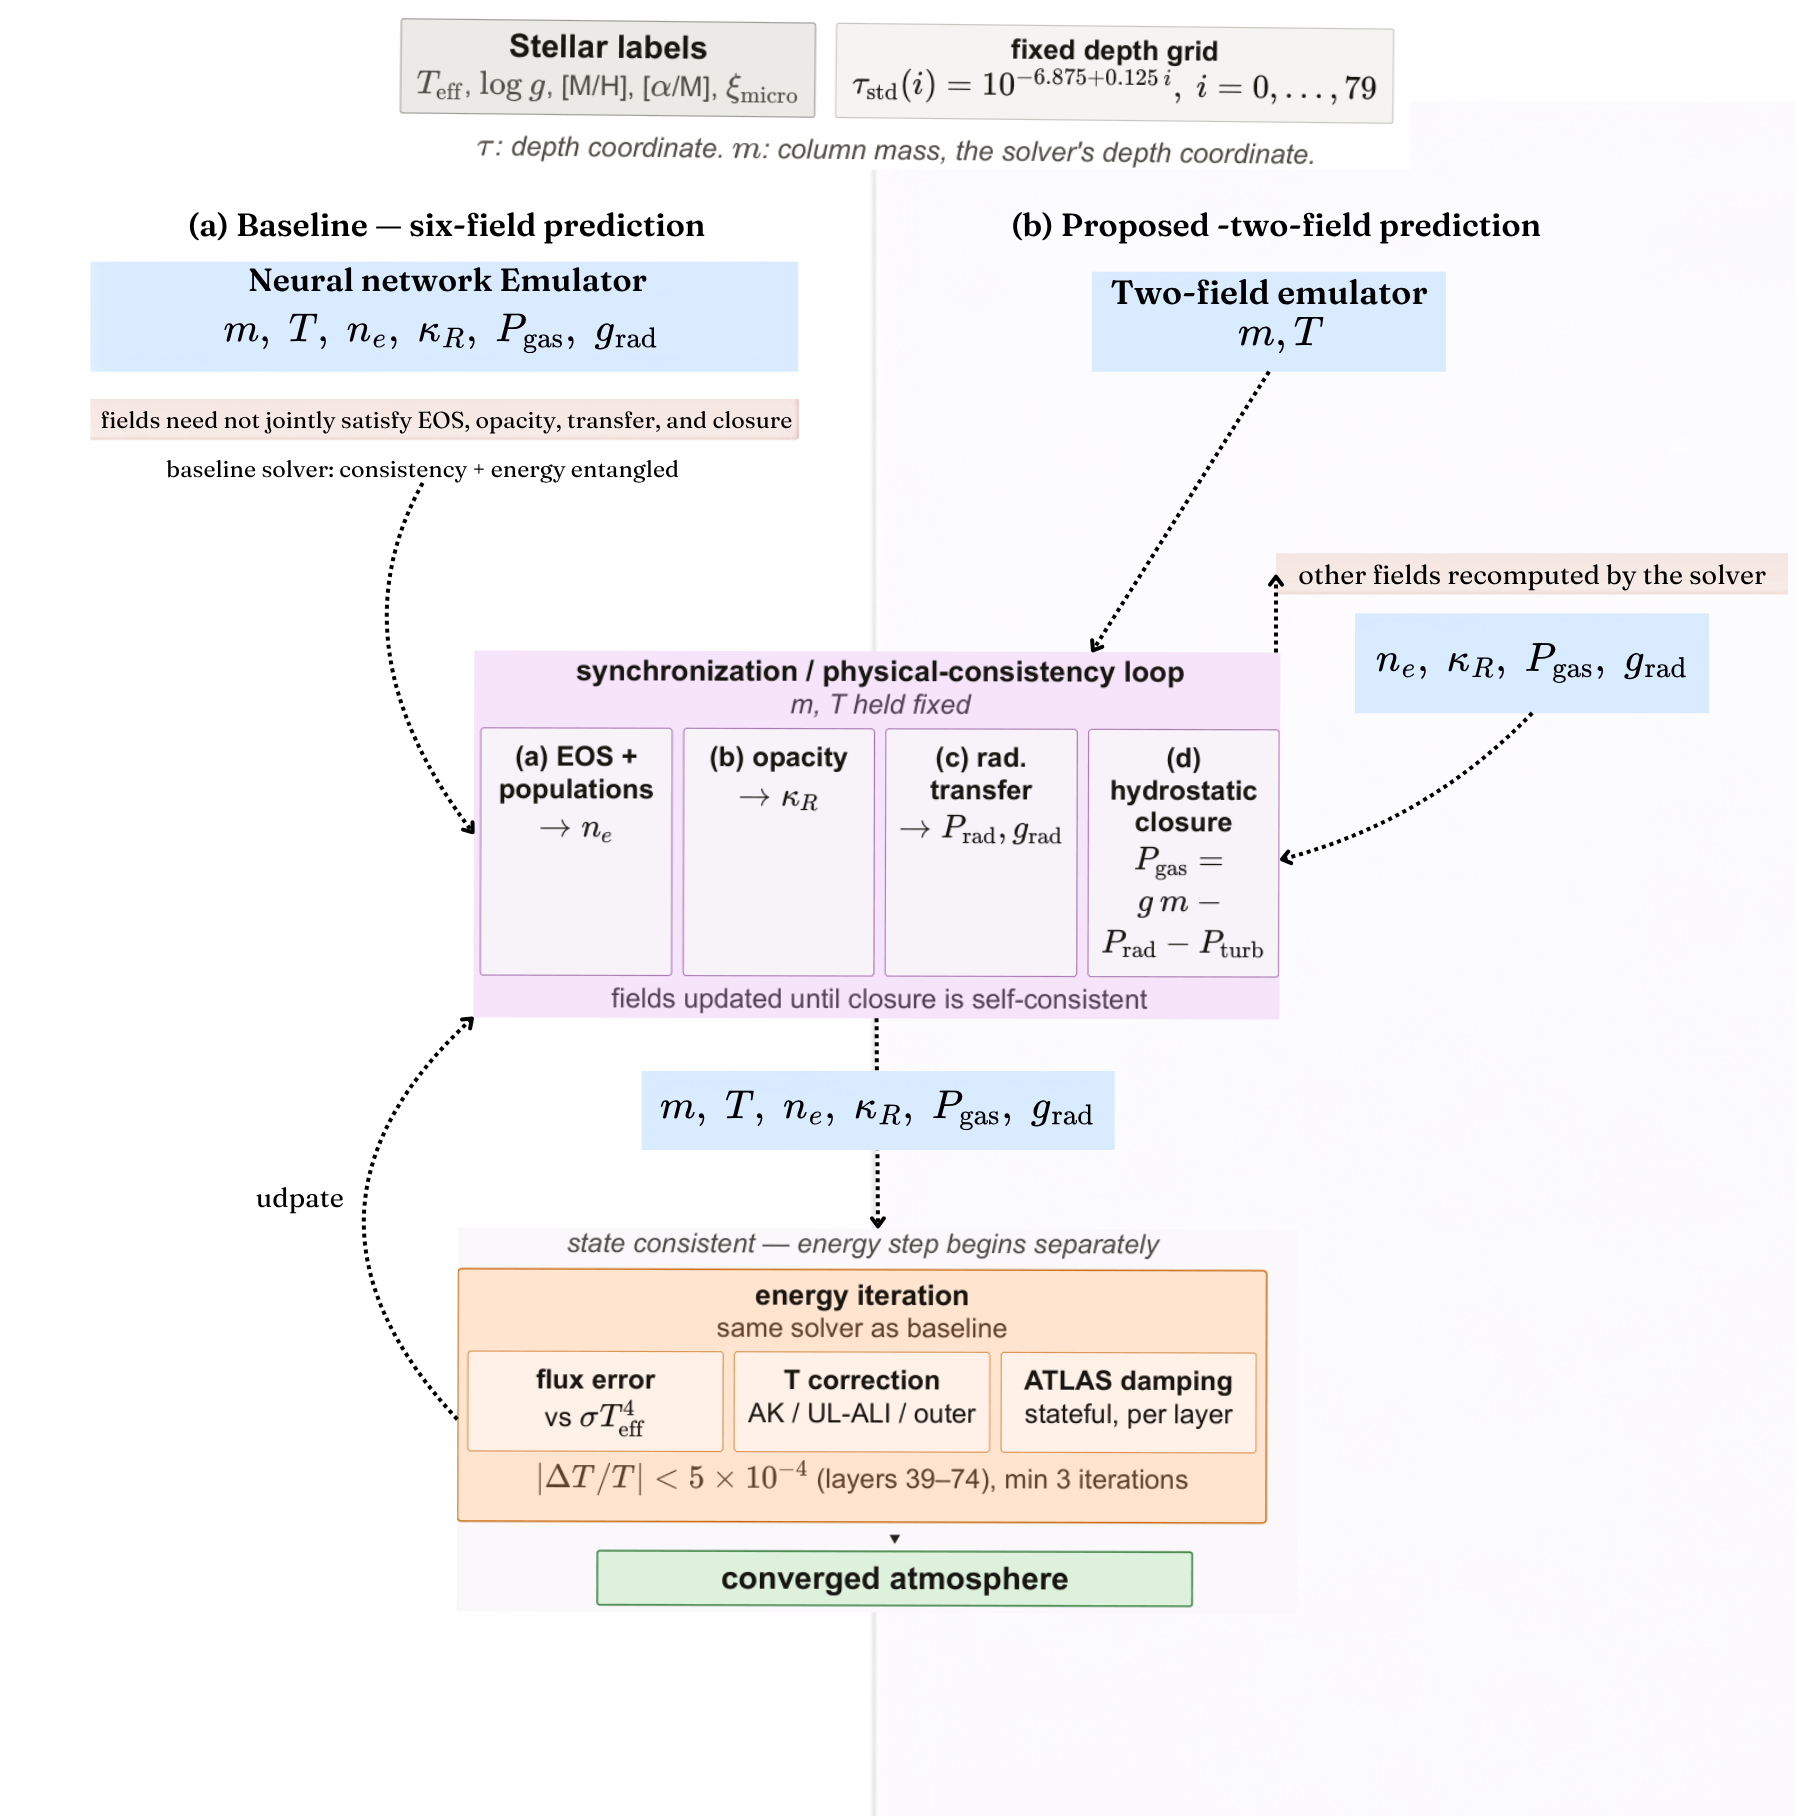
\includegraphics[width=\hsize]{fig_two_warm_starts_one_solver.png}
  \caption{Two warm starts feeding the same production solver. The released
    baseline predicts all six stored fields, whereas the proposed emulator
    predicts only $m$ and $T$. For the two-field arm, the equation of state,
    opacity, radiative transfer and hydrostatic closure synchronize
    $P_{\rm gas}$, $n_{\rm e}$, $\kappa_{\rm R}$ and $g_{\rm rad}$ at fixed
    $(m,T)$ before the unchanged energy iteration begins. The two-field arm
    needs no second predictor: the first synchronization pass is seeded from
    the labels and hydrostatic balance alone ($P_{\rm gas}=g\,m$, with
    positive $n_{\rm e}$ and $\kappa_{\rm R}$ placeholders and
    $g_{\rm rad}=0$), and subsequent passes recompute all four fields from the
    solver's own equation of state, opacity, transfer and closure routines.}
  \label{fig:state}
\end{figure*}

\subsection{Synchronization to self-consistency}
\label{sec:consistency}

The decisive implementation choice is to make the rebuilt state
self-consistent before the solver sees it. In the earlier two-field handoff
described in Sect.~\ref{sec:intro}, a single population/opacity/transfer
synchronization was applied and the ordinary iteration was then started; the
column mass in the most sensitive upper layer moved by about 13 per cent even
though converged temperature and mass profiles had been supplied. Since the
supplied profiles were exact, this displacement cannot be attributed to
prediction error: it indicates that the map itself has moved to a different
branch.

The mechanism lies in the coupling inside $\mathcal{F}$. The gas pressure is
corrected only once the transfer solution has supplied the radiation pressure,
whereas the opacities and populations that drive the transfer solution depend
on the pressure with which the pass began, so that a single pass through the
chain cannot be self-consistent. The residual inconsistency is then acted upon
by the solver's first temperature correction and by the grid remapping that
accompanies it, which displaces the column mass. The displacement appears at
the top of the atmosphere, where the optical-depth closure is seeded not by
quadrature but by the closed form
\begin{equation}
  \tau_{0} = \kappa_{0}\,m_{0},
  \label{eq:seed}
\end{equation}
which approximates $\int_{0}^{m_0}\kappa\,{\rm d}m$ by assuming $\kappa$ is
constant above the first grid point. Equation~(\ref{eq:seed}) is a convention
rather than a numerical approximation that improves with resolution; it
determines where the drift appears and why repairing the closure cannot remove
it. The record of the earlier attempt supports the same interpretation:
additional synchronization passes reduced the closure residual from $0.279$ to
$0.0034$\,dex while the branch drift remained unchanged, and reseeding the
surface radiation pressure had no effect.

The rematerialization of Sect.~\ref{sec:reduced} is designed to remove
precisely this failure mode. In the candidate path, synchronization continues
until the pass-to-pass change in gas pressure falls below $10^{-3}$\,dex; the
representation controls retain their recorded fixed-pass protocol. In both
cases $m$ and $T$ are pinned to the reduced state throughout, and the four
fields are read out on the production grid of Eq.~(\ref{eq:grid}) before any
temperature correction or remapping is applied.
Appendix~\ref{app:resolution} examines the two grid-side remedies directly and
shows that both a finer representation of the coordinates and a finer
quadrature fail to produce a systematic improvement.

\subsection{A monotone column-mass parameterization}

When the two coordinates come from a network rather than from a converged
atmosphere, one structural property has to be guaranteed rather than learned.
Column mass must increase monotonically with depth; a profile that does not is
rejected outright by the rematerialization, not merely degraded. The production
grid is uniform in $\log_{10}\tau$, with a spacing of $0.125$ dex. We predict a
positive increment in $\log_{10}m$ for each step on this grid:
\begin{equation}
  \ell_0 = a(\theta), \qquad
  \Delta\ell_j = \epsilon + \mathrm{softplus}\bigl(s_j(\theta)\bigr), \qquad
  \ell_j = \ell_0 + \sum_{k=1}^{j}\Delta\ell_k ,
  \label{eq:monotone}
\end{equation}
where $\ell_j=\log_{10}m_j$ and
$\mathrm{softplus}(x)=\log(1+e^x)$ is the smooth positive activation. The
network predicts the anchor $a(\theta)$ and the layer scores $s_j(\theta)$ from
the stellar labels $\theta$. The floor is $\epsilon=10^{-6}$ dex per layer, so
each increment is strictly positive. In the code, each score also includes a
fixed offset from the mean training-set increment. The cumulative sum makes
monotonicity structural. Section~\ref{sec:learned} gives the ablation that
justifies the cost of doing so.

% The compact non-neural initializer is retained as an appendix diagnostic rather
% than treated as a co-equal main-text result.
\section{Data and evaluation protocol}
\label{sec:data}

\subsection{Corpus and samples}

All experiments draw on \NcorpusStars\ converged solver-output atmospheres on the
grid of Eq.~(\ref{eq:grid}). The five-label support spans
$4000$--$10\,500$\,K in effective temperature, $0.7$--$5.3$ in $\log g$,
$-2.5$ to $+0.5$ in $[\rm M/H]$, $-0.1$ to $+0.5$ in
$[\alpha/\rm M]$, and $0.5$--$4.0$\,km\,s$^{-1}$ in microturbulence.
The learned model is trained on the corpus training split and assessed on a
development-60 sample excluded from training and validation. The sealed-200
holdout is disjoint from those rows and was fixed before the final policy was
opened. It is the only sample used to assess generalization.

The corpus contains only atmospheres that converged in fewer than thirty
iterations. Every convergence claim is therefore conditional on the region
already represented by this corpus; the experiments do not test whether a new
initializer rescues labels for which the solver fails from the outset.

\subsection{Initializers compared}

The main text compares three initializers. The released six-field network is the
Paper~I production baseline and predicts all six profiles directly. The learned
two-field initializer predicts only $m$ and $T$ and derives the remaining fields
through the solver-consistent rematerialization path. The sealed candidate is a
later frozen policy built on the same two-field representation and qualified on
development data before the sealed holdout was opened. Detailed asset records,
including the analytic comparison, are given in Appendix~\ref{app:assets}.
In the refreshed candidate-arm calculations, rematerialization starts from the
labels and hydrostatic balance, and no six-field-emulator checkpoint is queried
at inference. This is runtime independence, not training independence: the
training targets are converged full atmospheres, and the frozen policy was
qualified against products from the production arm.
It is also not exact numerical seed invariance: the adaptive stop is applied
to pressure, so the other rematerialized fields can retain differences of
order the stated synchronization tolerance.

\subsection{Evaluation protocol}

We evaluate each candidate at three levels. The profile level compares
$(m,T)$ with the converged truth. The solver level restarts the unmodified
solver and records convergence, iteration count, contraction and
non-monotonic trajectories. The spectral level compares converged products over
\NgateWindowLo--\NgateWindowHi\,nm at $R=\NgateResolution$, using the reference
gate implementation and the acceptance bar \NgateBar. Because the solver's
converged product depends on its starting state, the bar is calibrated against
the production retry start; the control and full metric definitions are given
in Appendix~\ref{app:gates}.
\section{Results}
\label{sec:results}

The representation and learned-initializer results below use the
development-\NevalStars\ sample, which was available throughout the
construction of the method; the original sealed-200 opening is the only
measurement that bears on generalization. Every development artifact that
executes rematerialization was regenerated from the physical seed for this
paper revision; the frozen two-field predictions and the released six-field
comparison products were not changed.

\subsection{Representation sufficiency}
\label{sec:sufficiency}

We first show that two fields are sufficient to carry the state, removing the
predictor from the question entirely: taking the converged $(m,T)$ profiles of
each evaluation star, we discard the other four fields and rebuild them
through $\mathcal{F}$. This isolates the representation question from the
separate question of whether a network can predict the coordinates.

Table~\ref{tab:reconstruction} and Fig.~\ref{fig:fields} give the resulting
comparison. The four rebuilt fields agree with the values to which the solver
itself converged at $10^{-3}$ or better in the median. The error is smallest
through the middle of the atmosphere and rises toward both boundaries, and a
handful of individual layers in a handful of stars reach tens of percent,
always at the extreme top or bottom of the grid.

% Generated by paper/collect_numbers.py -- do not edit by hand.
\begin{table}
\caption{Relative errors of the four dependent fields reconstructed from the converged column-mass and temperature profiles, evaluated over \NevalStars\ stars and \NgridLayers\ depth points.}
\label{tab:reconstruction}
\centering
\setlength{\tabcolsep}{3.5pt}
\small
\begin{tabular}{lrrr}
\hline\hline\noalign{\smallskip}
Field & Median & $p_{90}$ & Maximum \\
\noalign{\smallskip}\hline\noalign{\smallskip}
Gas pressure $P_{\mathrm{gas}}$ & \ensuremath{4.05\times10^{-4}} & \ensuremath{3.23\times10^{-3}} & \ensuremath{3.60\times10^{-1}} \\
Electron density $n_{\mathrm{e}}$ & \ensuremath{5.67\times10^{-4}} & \ensuremath{3.71\times10^{-3}} & \ensuremath{2.92\times10^{-1}} \\
Rosseland opacity $\kappa_{\mathrm{R}}$ & \ensuremath{8.74\times10^{-4}} & \ensuremath{5.66\times10^{-3}} & \ensuremath{1.36\times10^{-1}} \\
Radiative acceleration $g_{\mathrm{rad}}$ & \ensuremath{8.47\times10^{-4}} & \ensuremath{4.53\times10^{-3}} & \ensuremath{2.28\times10^{-1}} \\
\noalign{\smallskip}\hline
\end{tabular}
\end{table}



A more demanding test is whether the solver accepts the rebuilt atmosphere as
a starting state. Table~\ref{tab:oracle} restarts the unmodified solver from
the rebuilt state and, for comparison, from the full six-field truth; both
converge on every star. The rebuilt state takes \NoracleIterMean\ iterations
against \NsixIterMean, and \NoracleAtFloor\ of \NevalStars\ stars reach
the three-iteration floor exactly, against \NsixAtFloor.
\NoracleGapStars\ stars show a gap, never exceeding \NoracleGapMax\ additional
iterations, and none fails. This gap is the honest measure of the regime in
which two fields remain distinguishable from six.

% Generated by paper/collect_numbers.py -- do not edit by hand.
\begin{table*}
\caption{Restarting the unmodified solver from an atmosphere rebuilt from the two coordinates alone, against one that kept all six fields. Both arms begin inside the convergence threshold, so their $q$ and non-monotonic fractions describe noise-floor behavior and must not be compared with arms that start an order of magnitude further out (Sect.~\ref{sec:learned}). The last column counts stars held only by the three-iteration floor.}
\label{tab:oracle}
\centering
\begin{tabular}{lrrrrrrr}
\hline\hline\noalign{\smallskip}
Restart from & Conv. & Iterations & $p_{90}$ & $q$ & Non-mono. & First residual & At floor \\
\noalign{\smallskip}\hline\noalign{\smallskip}
Converged $(m,T)$ + physics & 100\% & 3.37 & 3 & 0.650 & 30.0\% & \ensuremath{4.20\times10^{-4}} & 55 \\
Full six-field truth & 100\% & 3.23 & 3 & 0.637 & 31.7\% & \ensuremath{4.23\times10^{-4}} & 57 \\
\noalign{\smallskip}\hline
\end{tabular}
\end{table*}


Two cautions apply to Table~\ref{tab:oracle}, both visible in its last
column. The first concerns the floor: with almost every star already at three
iterations, the table has very little power to distinguish the arms, and the
difference between \NoracleIterMean\ and \NsixIterMean\ should not be
over-interpreted. The second is more consequential. Both arms begin at a
first-iteration residual of about \NoracleFirstResidual, already inside the
$5\times10^{-4}$ convergence threshold, so their contraction ratios and
non-monotonic fractions describe how the solver behaves at its noise floor
rather than how it contracts; they must not be compared with arms that start
an order of magnitude further from the fixed point.
Section~\ref{sec:learned} maintains this separation throughout.

Iteration counts and profile errors are both internal to the atmosphere; the
observable question is whether the reduced state changes the emergent
spectrum. This is where a representation claim can fail silently, since an
atmosphere can be inaccurate in a way that costs no iterations yet still
shifts the flux. Comparing the converged product of the rebuilt arm with that
of the six-field arm over \NgateWindowLo--\NgateWindowHi\,nm, we find that
the normalized flux differs by a median of \NtruthGateMedian, with a maximum
of \NtruthGateMax\ and \NtruthGateOver\ of \NtruthGateStars\ stars above
the bar, corresponding to a median roughly \NtruthGateFactor\ times below
it. Total flux and continuum behave in the same way
(Table~\ref{tab:spectral}, first row). Figure~\ref{fig:representation-spectra}
shows this comparison directly across the label support, including the star
with the largest normalized-flux difference. Four of the six stored fields can
therefore be discarded and rebuilt without any spectroscopically measurable
change to the star.

\begin{figure*}[t]
  \centering
  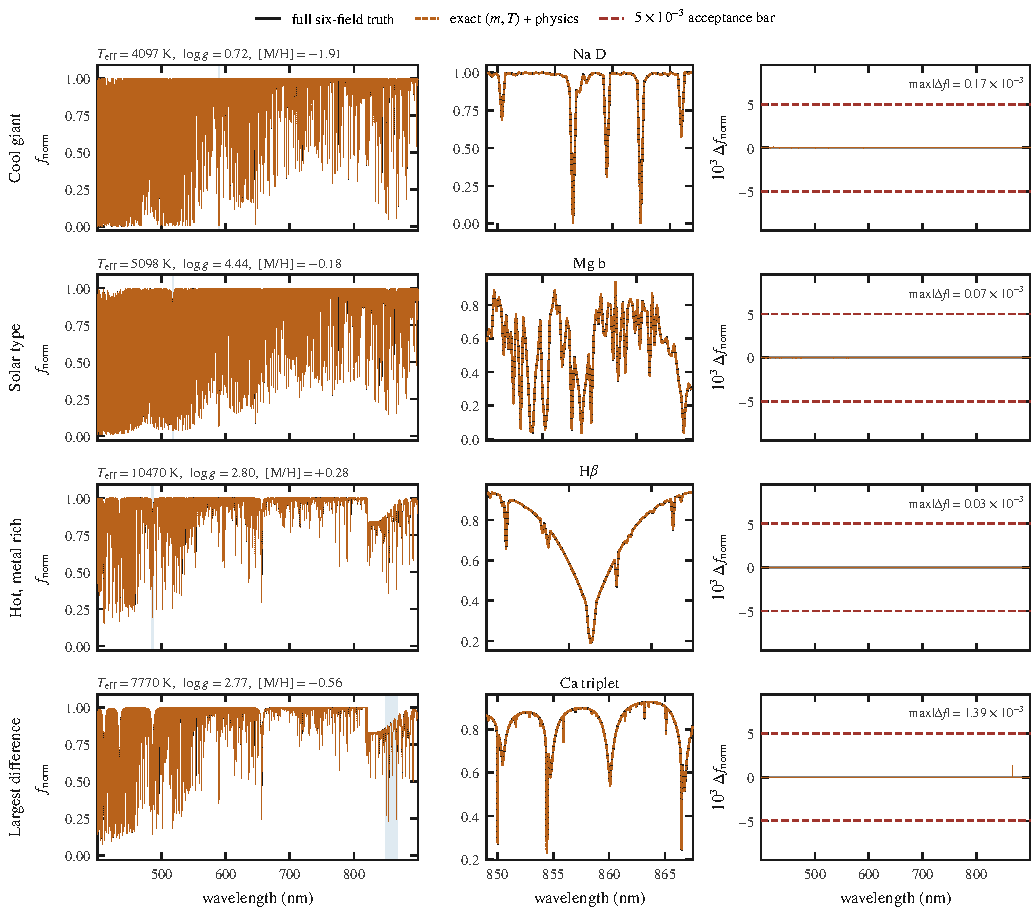
\includegraphics[width=\hsize]{fig_spectra.pdf}
  \caption{Representative converged spectra for the exact two-field
    representation test. The black curves start from the full six-field truth;
    the orange curves start after discarding four fields and rebuilding them
    from the same exact $(m,T)$ coordinates through the solver's physical
    closure. Both arms are then converged by the unchanged production solver
    and synthesized identically. The left column shows the full
    \NgateWindowLo--\NgateWindowHi\,nm gate window, the middle column resolves
    one diagnostic feature, and the right column shows the normalized-flux
    difference against the \NgateBar\ acceptance bar. The rows span the tested
    label support; the bottom row is the largest normalized-flux difference
    among all \NtruthGateStars\ stars.}
  \label{fig:representation-spectra}
\end{figure*}

% The grid and top-boundary controls are reported in Appendix~\ref{app:resolution};
% they are diagnostic limits rather than a separate main-text result.

\subsection{A learned two-field emulator}
\label{sec:learned}

We next replace the converged coordinates with the learned two-field initializer. The
network maps the five stellar labels to $(\log_{10}m,\log_{10}T)$ on the
production grid and uses the monotone decoder of Eq.~(\ref{eq:monotone}).
Training and implementation details are recorded in Appendix~\ref{app:assets}.

The two-field emulator is more accurate than the released network in the median
for the shared coordinates, although the comparison inverts in the tail: its
$p_{95}$ temperature error is
\NlearnedTempPfive\ against \NprodTempPfive, and $p_{95}$ column-mass error
\NlearnedMassPfive\,dex against \NprodMassPfive\,dex.

More importantly, the emulator is also more accurate on the four fields it
never predicts. Table~\ref{tab:fields} and Fig.~\ref{fig:fields} compare the
four dependent fields obtained in the three ways on the same requested
held-out sample; the learned-field distribution is conditional on successful
physical rematerialization:
predicting two fields and deriving the remaining four improves on predicting
all six directly by factors of \NfieldGainLow\ to \NfieldGainHigh, field by
field. Two predicted fields completed by the solver's physics thus outperform
six directly predicted fields across the entire state.

% Generated by paper/collect_numbers.py -- do not edit by hand.
\begin{table*}
\caption{Median relative error of the four dependent fields over the development sample and \NgridLayers\ layers. The learned row uses its \NderivedLearnedStars\ successful rematerializations; \NderivedLearnedFailures\ reconstruction failure is retained in the solver accounting but has no dependent-field profile to score. The second row is the primary comparison against the first: two predicted fields plus physics beat six predicted fields on every one of them. The third row is an oracle and bounds what the physics path alone can deliver, which localizes the entire remaining gap in the two-field predictor. All three rows use the same requested held-out sample, and the first two use the same checkpoints as Table~\ref{tab:learned}.}
\label{tab:fields}
\centering
\begin{tabular}{lrrrr}
\hline\hline\noalign{\smallskip}
Source of the four fields & $P_{\mathrm{gas}}$ & $n_{\mathrm{e}}$ & $\kappa_{\mathrm{R}}$ & $g_{\mathrm{rad}}$ \\
\noalign{\smallskip}\hline\noalign{\smallskip}
Six fields predicted directly & \ensuremath{1.81\times10^{-2}} & \ensuremath{1.30\times10^{-2}} & \ensuremath{1.43\times10^{-2}} & \ensuremath{3.18\times10^{-2}} \\
Learned two-field $(m,T)$ + physics & \ensuremath{4.51\times10^{-3}} & \ensuremath{5.24\times10^{-3}} & \ensuremath{5.21\times10^{-3}} & \ensuremath{5.59\times10^{-3}} \\
Converged $(m,T)$ + physics & \ensuremath{4.05\times10^{-4}} & \ensuremath{5.67\times10^{-4}} & \ensuremath{8.74\times10^{-4}} & \ensuremath{8.47\times10^{-4}} \\
\noalign{\smallskip}\hline
\end{tabular}
\end{table*}


\begin{figure*}[t]
  \centering
  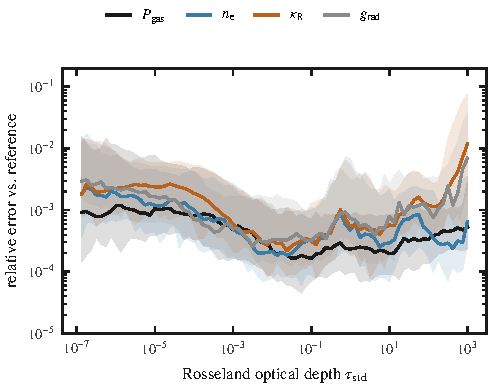
\includegraphics[width=0.48\hsize]{fig_reconstruction.pdf}\hfill
  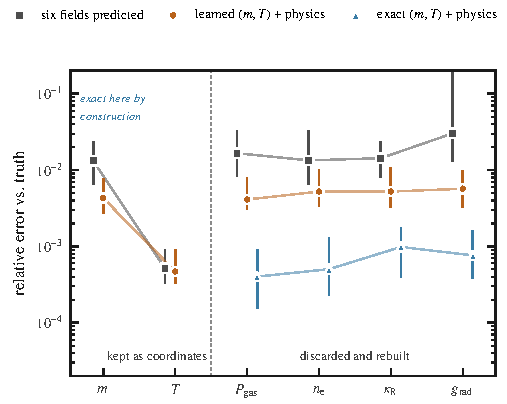
\includegraphics[width=0.48\hsize]{fig_fields.pdf}
  \caption{Field reconstruction and learned prediction on the same requested
    \NevalStars\ held-out stars. The learned dependent-field summaries contain
    the \NderivedLearnedStars\ stars that rematerialized successfully; the
    remaining \NderivedLearnedFailures\ failure has no full profile to score.
    \emph{(a)} Relative errors of the four fields
    rebuilt from the converged $(m,T)$ profiles, showing the floor set by the physical closure.
    \emph{(b)} Median errors for all six fields when the released network
    predicts all six directly, when the learned initializer predicts only
    $(m,T)$, and when $(m,T)$ are taken from the converged atmosphere. The two-field path derives the four
    dependent fields more accurately than the released network, while the
    converged coordinates show the residual floor of the physics path.}
  \label{fig:fields}
\end{figure*}

The converged-coordinate arm sets the floor imposed by the physics path; the
learned arm adds the error of predicting the two coordinates.

Table~\ref{tab:learned} and Fig.~\ref{fig:convergence} give the comparison
most relevant for initialization. Against the released initializer on the
same stars under the same policy, the learned two-field start reduces the
mean iteration count from \NprodIterMean\ to \NlearnedIterMean\ --- a
reduction of \NiterReduction\ --- improves the contraction ratio from
\NprodQ\ to \NlearnedQ, and cuts the fraction of non-monotonic
trajectories from \NprodNonmono\ to \NlearnedNonmono. All three arms in
that table begin at a comparable distance from the fixed point, so unlike
Table~\ref{tab:oracle} the contraction columns are directly comparable.

% Generated by paper/collect_numbers.py -- do not edit by hand.
\begin{table*}
\caption{Convergence from three initializations on the same \NevalStars\ development stars. All begin at comparable initial residuals, so their contraction statistics can be compared directly. The learned two-field model is the \NnetDepth$\times$\NnetWidth\ monotone network described in Sect.~\ref{sec:learned}; the independently tested model in Table~\ref{tab:blind} includes the radial-basis corrections of Sect.~\ref{sec:learned}.}
\label{tab:learned}
\centering
\begin{tabular}{lrrrrrrr}
\hline\hline\noalign{\smallskip}
Restart from & Conv. & Iterations & $p_{90}$ & $p_{99}$ & $q$ & Non-mono. & First residual \\
\noalign{\smallskip}\hline\noalign{\smallskip}
Six-field initializer & 98.3\% & 5.59 & 8 & 11.26 & 0.656 & 53.3\% & \ensuremath{2.44\times10^{-3}} \\
Learned two-field + physics & 93.3\% & 4.05 & 6 & 8.45 & 0.547 & 18.6\% & \ensuremath{2.75\times10^{-3}} \\
Six-field, alternate converged start & 93.3\% & 7.45 & 10 & 12.00 & 0.658 & 78.3\% & \ensuremath{6.75\times10^{-3}} \\
\noalign{\smallskip}\hline
\end{tabular}
\end{table*}


\begin{figure*}[t]
  \centering
  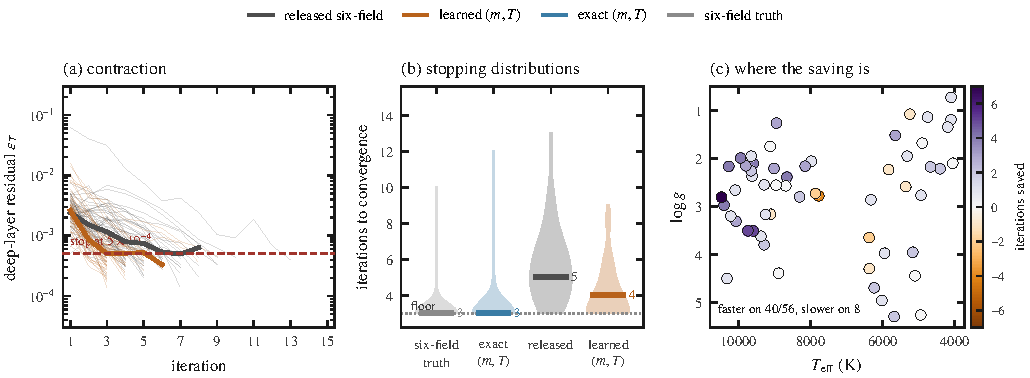
\includegraphics[width=\hsize]{fig_convergence.pdf}
  \caption{The learned two-field start on the unmodified solver. \emph{(a)}
    The deep-layer residual of Eq.~(\ref{eq:stop}) against iteration number:
    thin lines are individual stars, thick lines the median over the stars
    still iterating, drawn only while at least eight remain. The learned start
    enters the threshold sooner and with less of the oscillation that keeps the
    released start above it. \emph{(b)} Stopping distributions for the compared
    starts, with medians marked; the dotted line is the three-iteration floor.
    \emph{(c)} The paired
    per-star saving in label space. Purple is where the learned start costs
    fewer iterations than the released one, orange where it costs more. The
    saving is not uniform over the support: its Spearman correlation with
    $T_{\rm eff}$ is $\rho=\NlearnedGainRho$ ($p=\NlearnedGainP$), and above
    $9000$\,K it averages \NlearnedHotGain\ iterations against
    \NlearnedRestGain\ over the rest of the range.}
  \label{fig:convergence}
\end{figure*}

This improvement comes at a stated cost: the learned initializer fails on
\NlearnedFailures\ stars against the released initializer's \NprodFailures\ on
the same \NevalStars\ stars. The refreshed candidate count comprises
\NlearnedReconstructionFailures\ failures during physical rematerialization
and \NlearnedSolverFailures\ failures after restart. These are failures of the
complete learned-initializer path; the exact-coordinate experiment above
separately shows that they are not evidence against the sufficiency of the
two-field state itself.

The monotonicity ablation is reported in Appendix~\ref{app:assets}; the main
text uses the structurally monotone parameterization throughout.

% Generated by paper/collect_numbers.py -- do not edit by hand.
\begin{table*}
\caption{Normalized-flux differences between converged atmospheres over \NgateWindowLo--\NgateWindowHi\,nm at $R=\NgateResolution$. The \NgateBar\ value is retained as a common reference level, not as a universal acceptability boundary. Only stars with converged atmospheres from both initial states enter each row. The final row measures the start dependence of the reference solver and provides the numerical scale for the other comparisons.}
\label{tab:spectral}
\centering
\begin{tabular}{lrrrr}
\hline\hline\noalign{\smallskip}
Comparison & $N$ & Median & Maximum & Above reference \\
\noalign{\smallskip}\hline\noalign{\smallskip}
Converged $(m,T)$ vs.\ reference atmosphere & 60 & \ensuremath{8.28\times10^{-5}} & \ensuremath{1.39\times10^{-3}} & 0/60 \\
Learned two-field vs.\ six-field reference & 56 & \ensuremath{1.61\times10^{-3}} & \ensuremath{5.04\times10^{-3}} & 1/56 \\
Grey--convective vs.\ reference, development & 53 & \ensuremath{3.20\times10^{-2}} & \ensuremath{1.33\times10^{-1}} & 45/53 \\
Grey--convective vs.\ reference, post-hoc 200 & 179 & \ensuremath{2.59\times10^{-2}} & \ensuremath{1.70\times10^{-1}} & 150/179 \\
Six-field reference vs.\ alternate converged start & 56 & \ensuremath{3.44\times10^{-3}} & \ensuremath{1.50\times10^{-2}} & 16/56 \\
\noalign{\smallskip}\hline
\end{tabular}
\end{table*}


The converged-coordinate comparison lies far below the acceptance bar. The
learned comparison is close to the bar, but the production retry-start
control is larger by a factor of about two in the median and has more
exceedances. The candidate therefore changes the solver product less than the
solver's own accepted restart variability, although the control also
indicates that the spectral bar is not an absolute uniqueness test.

\subsection{Sealed blind test}
\label{sec:blind}

The results presented so far are development results. To test generalization,
we froze a complete policy on the reduced coordinates and only then opened a
200-star holdout that had been sealed in advance; neither the frozen
prediction nor the gate policy was tuned after it was opened. Because the
candidate had passed the three development gates before freezing, this test
evaluates transfer rather than another round of model selection.

The first opening used the historical six-field-emulator seed for the four
fields that rematerialization subsequently overwrites. After the holdout had
already been opened, we removed that runtime dependency and reran the unchanged
two-field prediction and solver from the physical seed described in
Appendix~\ref{app:remat}. The numerical values and orange curves below use this
post-opening rerun. It is an implementation confirmation on the previously
sealed sample, not a second blind test; the original gate outcomes are
unchanged.

The candidate did not transfer (Fig.~\ref{fig:blind}).
Table~\ref{tab:blind} gives the comparison with the development sample on
which the candidate had qualified. The profile gate fails on column mass,
with a $p_{95}$ of \NblindMassPfive\,dex against a limit of
\NblindMassLimit\,dex, and \NblindTempBlowouts\ temperature and
\NblindMassBlowouts\ column-mass blow-out stars, \NblindUnionBlowouts\ distinct
stars in all. The spectral gate fails as well, with \NblindSpecOver\ of
\NblindPaired\ paired stars above the bar and a maximum of \NblindSpecMax.

% Generated by paper/collect_numbers.py -- do not edit by hand.
\begin{table}
\caption{The frozen two-field candidate of Sect.~\ref{sec:blind} on the development sample used for qualification and on a 200-star holdout sealed before the policy was opened. The holdout values shown here come from the post-opening physical-seed rerun of the unchanged prediction and solver. They confirm that the gate outcome is not caused by querying the six-field checkpoint at inference, but they are not a second blind test. The iteration speed-up survives, while the profile and spectral reliability required for deployment does not.}
\label{tab:blind}
\centering
\setlength{\tabcolsep}{4.0pt}
\small
\begin{tabular}{lrr}
\hline\hline\noalign{\smallskip}
Quantity & Development & Holdout rerun \\
\noalign{\smallskip}\hline\noalign{\smallskip}
Stars & 60 & 200 \\
Temperature $p_{95}$ & \ensuremath{2.06\times10^{-3}} & \ensuremath{3.38\times10^{-3}} \\
Column mass $p_{95}$ (dex) & \ensuremath{1.19\times10^{-2}} & \ensuremath{2.66\times10^{-2}} \\
Profile blow-outs ($T$ / $m$) & 0 / 0 & 6 / 18 \\
Candidate usable products & 60/60 & 190/200 \\
Production usable products & 60/60 & 193/200 \\
Mean iterations, c.\ / p. & 3.77 & 4.12 / 5.69 \\
Normalised flux, max & \ensuremath{4.47\times10^{-3}} & \ensuremath{1.42\times10^{-2}} \\
Normalised flux, over bar & 0/60 & 25/188 \\
\noalign{\smallskip}\hline\noalign{\smallskip}
Outcome & pass & \textbf{fail} \\
\noalign{\smallskip}\hline
\end{tabular}
\end{table}


\begin{figure*}[t]
  \centering
  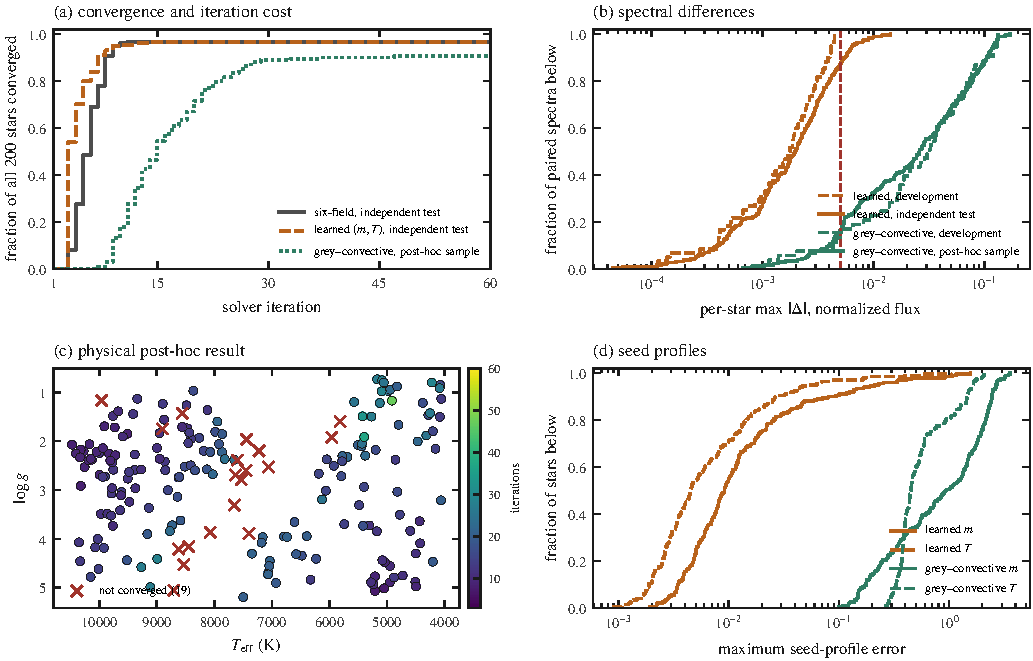
\includegraphics[width=\hsize]{fig_blind.pdf}
\caption{The previously sealed holdout, rerun after opening with the physical
    reconstruction seed. \emph{(a)} Iteration histograms on the same 200
    stars: two candidate reconstructions fail before restart; among the
    remaining 198, the frozen two-field candidate (orange) keeps its mode at
    the three-iteration floor, well ahead of the released initializer (grey).
    \emph{(b)} The spectral acceptance gate on the same frozen policy:
    cumulative per-star maximum normalized-flux difference on the development
    sample the candidate qualified on (dashed blue) and on the post-opening
    physical-seed rerun (orange), against the \NgateBar\ bar. The speed found
    at the original blind opening is reproduced; the spectral reliability
    still fails. \emph{(c)} The development-60 and holdout-200 samples in the
    $T_{\rm eff}$--$\log g$ plane. \emph{(d)} The holdout stars in the
    $[\mathrm M/\mathrm H]$--$\log g$ plane, marked
    by which gate each fails: profile blow-outs (red), spectral exceedances
    (orange), and solver or reconstruction failures (black), with that priority
    when a star fails more than one gate. The failures are not confined to one
    corner of the support.}
  \label{fig:blind}
\end{figure*}

What does survive the blind test is the speed advantage. On the
\NblindPaired\ paired usable products the candidate converges in
\NblindCandIters\ mean iterations against \NblindProdIters and reduces the
non-monotonic fraction from \NblindProdNonmono\ to \NblindCandNonmono. The
paired saving is \NblindPairedDiffMedian\ iterations in the median, with a
bootstrap 95 per cent interval of \NblindPairedDiffCiLo\ to
\NblindPairedDiffCiHi\ for the mean saving. The reliability does not
transfer: the blind spectral exceedance rate is \NblindSpecOver\ of
\NblindPaired\, and the candidate also produces fewer usable atmospheres
than the released initializer. The measured speed-up therefore remains a
demonstration rather than a production replacement.

%%%%%%%%%%%%%%%%%%%%%%%%%%%%%%%%%%%%%%%%%%%%%%%%%%%%%%%%%%%%%%%%%%%%%%%%%%%%%
\section{Discussion}
\label{sec:discussion}

The central result is structural rather than statistical. A six-field network can
make each field individually plausible while producing a state that violates
the relations enforced by the solver. Predicting only $(m,T)$ and deriving the
other fields instead gives the solver a coherent state. This explains why the
two-field initializer improves the dependent-field errors even though its
two predicted coordinates are not uniformly closer to truth. More importantly,
the learned start converges faster despite beginning with a larger first
residual. The tested profile metrics are therefore not basin certificates;
initialization objectives must ultimately be evaluated through the solver,
consistent with the broader idea of solver-in-the-loop optimization
\citep{um2020}.

These claims remain bounded. The corpus contains only converged atmospheres, the
baseline is the released rather than the best internal initializer, and the
reported iteration saving begins after the non-free rematerialization step.
The spectral gate measures flux agreement over one wavelength window and does
not test whether stellar labels are recovered by a downstream fit. The sealed
test confirms that the speed advantage transfers but that profile and spectral
reliability do not. The reduced representation is therefore validated as a
solver-consistent warm-start construction within the tested support, not as a
deployable replacement or a universal atmosphere model. The analytic
initializer and additional gate controls are retained as development
diagnostics in the appendix.

The remaining physical clue is at the top boundary. The resolution controls in
Appendix~\ref{app:resolution} show that refining the interior representation or
quadrature does not remove the hard tail, while the residual is concentrated in
the fixed surface seed. This makes the boundary condition the leading
hypothesis, not an established cause. Testing it requires atmospheres extending
above the current $\tau_{\rm min}$ and a direct change to the seed.
\section{Conclusions}
\label{sec:conclusions}

Within the tested five-label support and production solver branch, the
converged atmosphere can be represented by two coordinates, $m(\tau)$ and
$T(\tau)$. Rebuilding the other four fields through the solver's own physics
reproduces the converged structure to $10^{-3}$ or better in the median and
gives spectral agreement below the calibrated acceptance bar. The essential requirement is
synchronization at fixed $(m,T)$ before the ordinary temperature correction and
remapping begin.

The learned two-field initializer improves the dependent-field accuracy over
the released six-field network and reduces the mean iteration count from
\NprodIterMean\ to \NlearnedIterMean, with fewer non-monotonic trajectories. On
the sealed 200-star holdout, the speed advantage survives but the profile and
spectral gates fail. A post-opening rerun reproduces that outcome without
querying the six-field checkpoint in the candidate arm. We therefore report
the method as a validated representation and a promising warm-start
construction, not as a production initializer.

The most informative next experiment is therefore not a further interior grid
refinement or profile-loss ablation but a direct test of the upper boundary
condition, using atmospheres that extend above the current $\tau_{\rm min}$.

\begin{acknowledgements}
  Author contributions: J.~L. designed and ran the experiments, wrote the
  software and the manuscript. Y.-S.~T. contributed the reduced-coordinate idea
  the paper tests and the prior negative results that shaped its design, and
  made the earlier warm-start campaign available. Both authors reviewed the
  manuscript.
  % TODO: funding and computing-resource statements.
\end{acknowledgements}

\bibliographystyle{aa}
\bibliography{refs}

%%%%%%%%%%%%%%%%%%%%%%%%%%%%%%%%%%%%%%%%%%%%%%%%%%%%%%%%%%%%%%%%%%%%%%%%%%%%%
\begin{appendix}

\section{The rematerialization path}
\label{app:remat}

Given coordinates $m(\tau)$, $T(\tau)$ and labels $\theta$, the four dependent
fields are obtained by executing the following steps, all of them the solver's
own production routines on the grid of Eq.~(\ref{eq:grid}).

\begin{enumerate}
  \item \emph{Seed.} An atmosphere object is constructed carrying $m$ and $T$ on
    the production grid. The remaining fields are seeded from the labels and
    hydrostatic balance alone: $P_{\rm gas}=g\,m$, with positive $n_{\rm e}$
    and $\kappa_{\rm R}$ placeholders and $g_{\rm rad}=0$. The
    molecular equation of state and the first opacity and transfer passes
    overwrite these values, so they only fix where the synchronization starts;
    no second network is involved. A profile whose column mass is not strictly
    increasing is rejected here rather than repaired.
  \item \emph{Populations.} The equation of state is solved for the chemical
    populations and the electron density at each layer.
  \item \emph{Opacity.} Continuum and line opacities are evaluated and combined
    into the Rosseland mean $\kappa_{\rm R}$.
  \item \emph{Transfer.} The radiative transfer solution supplies the radiation
    pressure and the radiative acceleration $g_{\rm rad}$.
  \item \emph{Closure.} The gas pressure is recomputed from
    Eq.~(\ref{eq:hse}) with the radiation and turbulent terms now known.
\end{enumerate}

Steps 2--5 are repeated for a small number of synchronization passes, because a
single pass is not self-consistent: the populations and opacities of steps~2--3
are evaluated at the gas pressure the pass started with, and that pressure is
corrected only in step~5, from the radiation pressure they themselves imply.
The representation controls use \NsyncPasses\ fixed passes. Candidate-arm
solver runs use the adaptive path, with a limit of \NsyncMaxPasses\ passes and a
pressure-change tolerance of \NsyncPressureTolerance\,dex. A failure to meet
that tolerance is retained as a reconstruction failure rather than silently
accepted. $m$ and $T$ are not modified at any step, and the depth grid is not
resampled at any step.

\section{Acceptance gate definitions}
\label{app:gates}

\emph{Profile.} Pointwise relative error in temperature and pointwise absolute
error in $\log_{10} m$, against the converged truth, over all layers and stars.
A star is a blow-out if its maximum temperature error exceeds $10$ percent or
its maximum column-mass error exceeds $0.1$\,dex.

\emph{Solver.} The unmodified solver is restarted from the candidate state under
the production policy. We record the fraction of stars that converge; the
iteration count of the converging trial; the geometric mean of the ratio $q_k =
r_{k+1}/r_k$ of successive deep-layer temperature residuals; and the fraction of
trajectories on which $r_k$ is not monotonically decreasing. A product that
satisfies the temperature stopping rule but is not finite is counted as a
failure, not as a convergence.

\emph{Spectral.} Both arms' converged atmospheres are synthesized over
\NgateWindowLo--\NgateWindowHi\,nm at $R = \NgateResolution$ in double
precision. Three quantities are compared: the maximum absolute difference in
normalized flux; the maximum absolute difference in total flux, divided by the
continuum; and the maximum relative difference in the continuum. The acceptance
bar is \NgateBar\ on each. The production retry-start control in
Table~\ref{tab:spectral} provides the calibration needed to interpret this bar.

\section{Solver behavior by label sampling}
\label{app:baseline}

Table~\ref{tab:baseline} shows what the unmodified solver does when started
from the released six-field initializer. The solver and the initializer are
identical in all four rows; only the way in which the stellar labels are drawn
changes, and the resulting spread is the point of the comparison. Drawing
labels uniformly across the label ranges the corpus spans gives
\NboxConverged\ convergence and \NboxFailed\ outright failures, whereas
resampling the corpus's own label distribution gives \NiidConverged\
convergence, with a $90$th-percentile iteration count of \NiidPninety. The
failure rate is set by where in that range the requests fall, not by the
solver.

% Generated by paper/collect_numbers.py -- do not edit by hand.
\begin{table*}
\caption{Convergence from the Paper~I six-field initializer for different stellar-label distributions. The solver and initializer are identical in every row; only the sampling within the support of Sect.~\ref{sec:data} differs. \emph{Uniform box} draws each label uniformly over that support, which covers the box rather than the stellar locus and so includes combinations no real star occupies; \emph{IID from corpus} resamples whole corpus rows with replacement, preserving the joint distribution the initializer was trained on; \emph{label-box boundary} pins at least one label within 5\% of a face of that support; \emph{low gravity, metal poor} samples uniformly inside $\log g \in [0.7, 2.8]$, $[\rm M/H] \in [-2.5, -0.5]$. Iteration counts include converged calculations only; $q$ is the geometric-mean ratio of successive temperature residuals, with $q<1$ indicating contraction.}
\label{tab:baseline}
\centering
\begin{tabular}{lrrrrrrr}
\hline\hline\noalign{\smallskip}
Label sampling & $N$ & Converged & Failed & Iterations & $p_{90}$ & $q$ & Non-monotonic \\
\noalign{\smallskip}\hline\noalign{\smallskip}
Uniform box & 300 & 85.3\% & 14.7\% & 6.26 & 9 & 0.752 & 64.0\% \\
IID from corpus & 1000 & 99.2\% & 0.8\% & 5.86 & 8 & 0.644 & 56.6\% \\
Label-box boundary & 500 & 80.6\% & 19.4\% & 6.74 & 10 & 0.763 & 70.2\% \\
Low gravity, metal poor & 500 & 81.8\% & 18.2\% & 6.19 & 10 & 0.811 & 64.2\% \\
\noalign{\smallskip}\hline
\end{tabular}
\end{table*}


\section{Resolution and boundary controls}
\label{app:resolution}

The representation-resolution control round-trips converged $(m,T)$ curves through
intermediate optical-depth grids before rematerialization. The restart behavior
is nearly unchanged across the tested range, even when representation error
changes by several orders of magnitude. A separate quadrature control increases
the integration density by sixteen-fold while keeping the surface seed fixed;
the closure residual is unchanged. The residual therefore belongs to the fixed
top-boundary seed rather than to the interior grid spacing.

% Generated by paper/collect_numbers.py -- do not edit by hand.
\begin{table*}
\caption{The converged $(m,T)$ curves are round-tripped through an intermediate logarithmic optical-depth grid of $N$ points and back onto the atmosphere grid before physical reconstruction, so that only the fidelity of the representation changes. Representation error is the median relative error in column mass; $N=\NgridLayers$ is the identity. Restart behavior remains near the three-iteration floor across the scan.}
\label{tab:resolution}
\centering
\begin{tabular}{rrrrrrr}
\hline\hline\noalign{\smallskip}
$N$ & Repr. error & Conv. & Iterations & $p_{90}$ & $q$ & Non-mono. \\
\noalign{\smallskip}\hline\noalign{\smallskip}
40 & \ensuremath{3.08\times10^{-5}} & 98.3\% & 3.46 & 4 & 0.554 & 15.0\% \\
80 & \ensuremath{<10^{-14}} & 100.0\% & 3.37 & 3 & 0.650 & 30.0\% \\
160 & \ensuremath{3.95\times10^{-7}} & 98.3\% & 3.19 & 3 & 0.657 & 30.0\% \\
320 & \ensuremath{4.72\times10^{-8}} & 98.3\% & 3.22 & 3 & 0.659 & 30.0\% \\
640 & \ensuremath{6.55\times10^{-9}} & 100.0\% & 3.35 & 3 & 0.649 & 30.0\% \\
\noalign{\smallskip}\hline
\end{tabular}
\end{table*}

% Generated by paper/collect_numbers.py -- do not edit by hand.
\begin{table*}
\caption{Optical-depth closure residual in the top five layers as the quadrature grid is refined, using the solver's own integrator and holding $\tau_{\mathrm{min}}$ fixed so that spacing is isolated from the boundary. Sixteen times the grid density moves the worst case in the fourth decimal place, because layer~0 involves no quadrature at all.}
\label{tab:continuity}
\centering
\begin{tabular}{lrrrrrr}
\hline\hline\noalign{\smallskip}
Refinement & Points & \multicolumn{3}{c}{Closure residual (dex)} & \multicolumn{2}{c}{Mass drift (\%)} \\
& & Median & $p_{99}$ & Max & $p_{99}$ & Max \\
\noalign{\smallskip}\hline\noalign{\smallskip}
$\times1$ & 80 & 0.00059 & 0.03571 & 0.66143 & 7.72 & 72.42 \\
$\times2$ & 159 & 0.00076 & 0.03507 & 0.66143 & 7.59 & 72.42 \\
$\times4$ & 317 & 0.00080 & 0.03504 & 0.66143 & 7.46 & 72.42 \\
$\times8$ & 633 & 0.00081 & 0.03498 & 0.66143 & 7.42 & 72.42 \\
$\times16$ & 1265 & 0.00081 & 0.03497 & 0.66143 & 7.42 & 72.42 \\
\noalign{\smallskip}\hline
\end{tabular}
\end{table*}


\begin{figure*}[t]
  \centering
  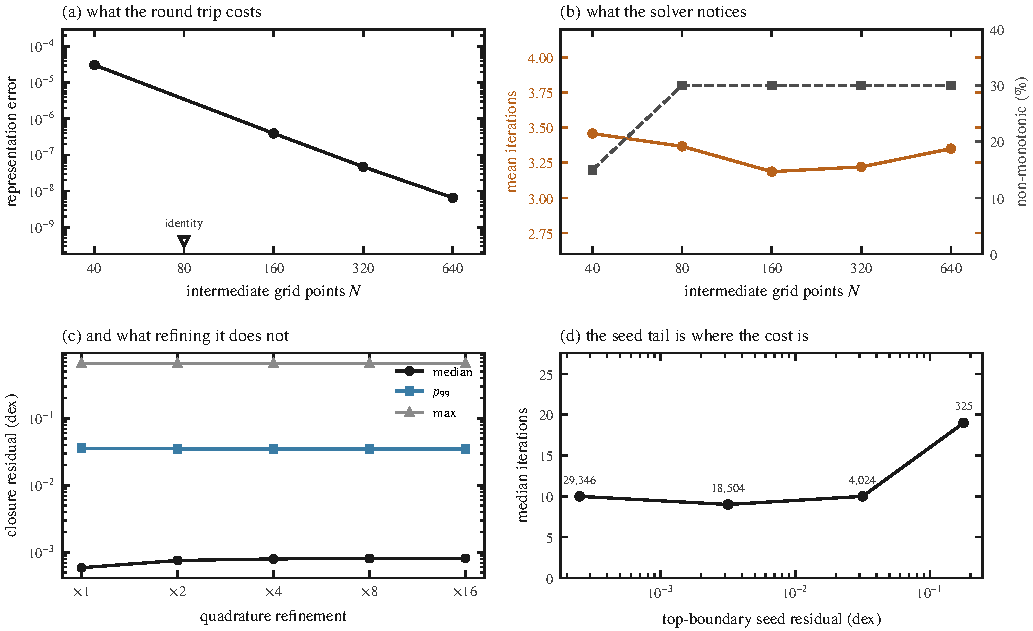
\includegraphics[width=\hsize]{fig_resolution.pdf}
  \caption{Resolution and boundary controls. Refining the intermediate
    representation or the quadrature does not change restart behavior or the
    top-layer closure residual. The hard tail is associated with the fixed
    surface seed, not with insufficient interior sampling.}
  \label{fig:resolution}
\end{figure*}

\section{Analytic initializer and additional diagnostics}
\label{app:analytic}

The analytic diagnostic replaces the neural checkpoint with a low-rank formula
for a grey-normalized temperature residual and $\log_{10}\kappa_{\rm R}$.
Column mass is then obtained by integrating
${\rm d}m/{\rm d}\tau=1/\kappa_{\rm R}$. The formula is fitted to the same
atmosphere family but is evaluated only on the development sample; it has no
spectral or sealed-holdout result. We retain it here as evidence that a compact
non-neural warm start can enter the solver basin, not as a competing main-text
method.

% Generated by paper/collect_numbers.py -- do not edit by hand.
\begin{table*}
\caption{Parameter structure of the analytic-parity formula. Each closure uses three effective-temperature regimes and 56 complete cubic label terms per regime. The two closures share the same five-label centering and scaling. Negative storage denotes deduplication, not a fitted correction; the total is the logical float count when the shared normalization is counted once.}
\label{tab:analytic-structure}
\centering
\setlength{\tabcolsep}{4.0pt}
\small
\begin{tabular}{llrrrrr}
\hline\hline\noalign{\smallskip}
Component & Fitted target & Label degree & Modes & Mean degree & Mode degree & Logical floats \\
\noalign{\smallskip}\hline\noalign{\smallskip}
Temperature & $\log_{10}(T/T_{\rm grey})$ & 3 & 5 & 22 & 18 & 1209 \\
Opacity & $\log_{10}\kappa_{\rm R}$ & 3 & 5 & 18 & 18 & 1197 \\
Shared label scaling & --- & --- & --- & --- & --- & -10 \\
Support and guards & --- & --- & --- & --- & --- & 11 \\
\textbf{Total} & --- & --- & --- & --- & --- & \textbf{2407} \\
\noalign{\smallskip}\hline
\end{tabular}
\end{table*}

% Generated by paper/collect_numbers.py -- do not edit by hand.
\begin{table*}
\caption{The learned and non-neural analytic initializers on the same development-60 stars. Profile errors are pooled over all $\NevalStars\times\NgridLayers$ layer values. Formal post-handoff iteration statistics use only converged stars; successfully constructed starts receive one trial of at most \NanalyticIterationLimit\ iterations, while a pre-handoff rematerialization failure counts as a non-convergence. This is not end-to-end timing. The solver records come from separate campaigns, not one contemporaneous executable. The learned count includes its trainable weights and stored standardization arrays. The analytic count is the current NPZ's float-entry count; it exceeds the \NanalyticConstants\ logical count by ten because the shared label normalization is repeated for the two closures. Deterministic integer exponent tables contribute \NanalyticIntegerEntries\ additional structural entries and are not counted as floating entries. Timeouts are counted as non-convergences. The analytic arm has no spectral or sealed-blind evaluation.}
\label{tab:analytic}
\centering
\setlength{\tabcolsep}{4.0pt}
\small
\begin{tabular}{llrrrrrr}
\hline\hline\noalign{\smallskip}
Initializer & Fitted profiles & Float entries & $T$ $p_{95}$ & $\log m$ $p_{95}$ & Converged & Mean iter. & Median \\
\noalign{\smallskip}\hline\noalign{\smallskip}
Learned two-field + physics & $(m,T)$ & 873\,450 & \ensuremath{3.74\times10^{-3}} & \ensuremath{1.52\times10^{-2}} & 56/60 & 4.05 & 4.0 \\
Analytic-parity formula & $(\delta_T,\log\kappa_{\rm R})\rightarrow m$ & 2\,417 & \ensuremath{1.91\times10^{-2}} & \ensuremath{8.76\times10^{-2}} & 57/60 & 7.77 & 8.0 \\
\noalign{\smallskip}\hline
\end{tabular}
\end{table*}

% Generated by paper/collect_numbers.py -- do not edit by hand.
\begin{table}
\caption{Column-mass parameterization, both arms trained identically for \NnetEpochs\ epochs on the same split and seed. The direct arm is genuinely the more accurate of the two and is still the one that has to be discarded: the profiles it rejects are rejected outright, not degraded.}
\label{tab:monotone}
\centering
\setlength{\tabcolsep}{4.0pt}
\small
\begin{tabular}{lrrr}
\hline\hline\noalign{\smallskip}
Parameterisation & $T$ $p_{95}$ & $\log m$ $p_{95}$ & Rejected \\
\noalign{\smallskip}\hline\noalign{\smallskip}
Monotone, Eq.~(\ref{eq:monotone}) & \ensuremath{3.74\times10^{-3}} & \ensuremath{1.52\times10^{-2}} & 0/60 \\
Direct, \NgridLayers\ outputs & \ensuremath{3.22\times10^{-3}} & \ensuremath{1.40\times10^{-2}} & 3/60 \\
\noalign{\smallskip}\hline
\end{tabular}
\end{table}


\begin{figure*}[t]
  \centering
  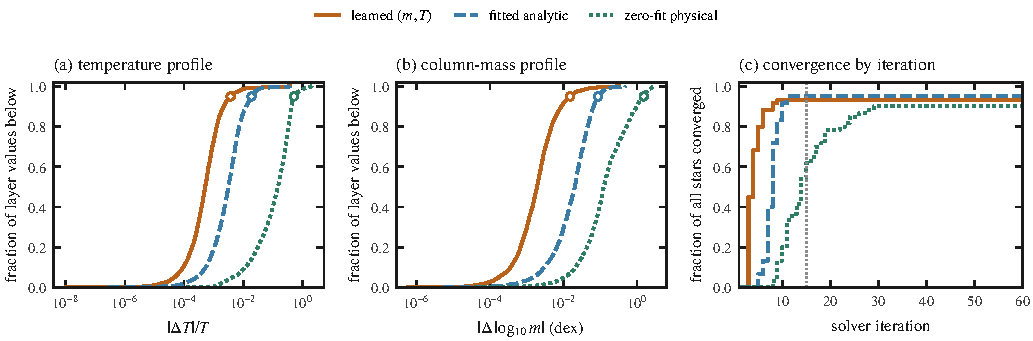
\includegraphics[width=\hsize]{fig_analytic.pdf}
  \caption{Development-set comparison of the learned and analytic initializers.
    The analytic formula has larger profile errors and is not evaluated by the
    spectral or sealed gates.}
  \label{fig:analytic}
\end{figure*}

\begin{figure*}[t]
  \centering
  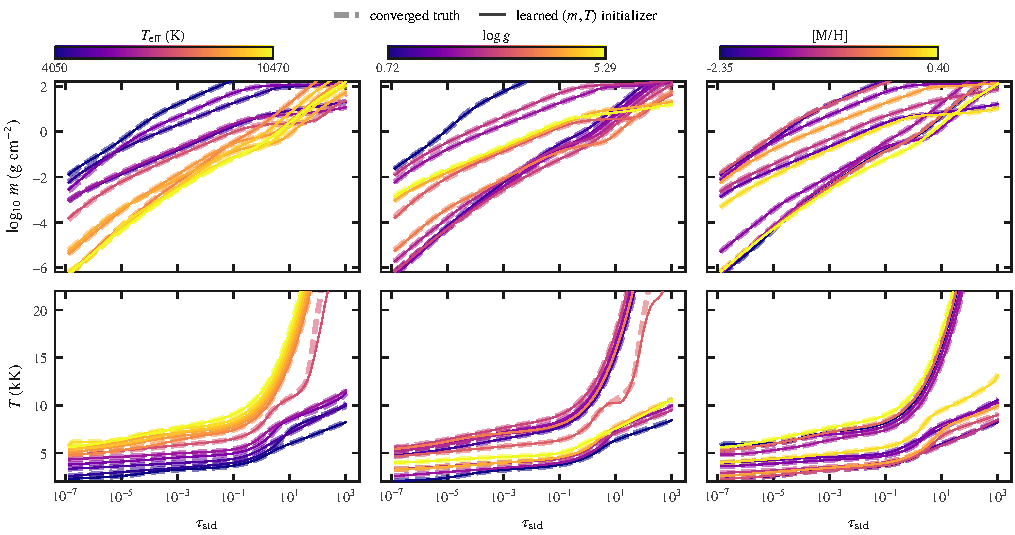
\includegraphics[width=\hsize]{fig_profiles.pdf}
  \caption{Additional profiles from the learned two-field initializer.}
  \label{fig:profiles}
\end{figure*}

\begin{figure*}[t]
  \centering
  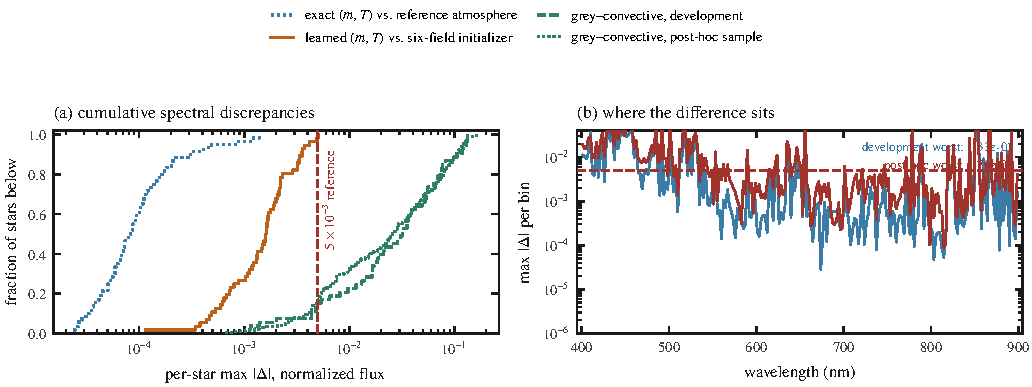
\includegraphics[width=\hsize]{fig_spectral.pdf}
  \caption{Additional spectral-gate diagnostics for the development sample and
    the production retry-start control.}
  \label{fig:spectral}
\end{figure*}

\section{Implementation and asset records}
\label{app:assets}

The following generated table records the initializer families, training roles
and frozen assets used by the experiments. These implementation details are
kept outside the main argument so that the scientific comparison remains
readable and auditable.

% Generated by paper/collect_numbers.py -- do not edit by hand.
\begin{table*}
\caption{The four initializer families compared in this paper. The released six-field network is the Paper~I production model and predicts all six fields directly; the two-field emulator predicts only the two coordinates and derives the rest through the physics path; the analytic-parity arm replaces the neural checkpoint by a compact formula for temperature and opacity and integrates column mass; the frozen blind candidate adds a bounded one-step solver correction and a local rescue term on top of a retrained two-field base. $^{\dagger}$The candidate is a three-component policy; the hash listed is its two-field base checkpoint, and the adapter hashes are recorded in the frozen-policy artifact. Hashes are the first 12 hexadecimal digits of the SHA-256 of the checkpoint file; full values are in \texttt{paper/numbers.json}.}
\label{tab:families}
\centering
\setlength{\tabcolsep}{3.5pt}
\footnotesize
\begin{tabular}{>{\raggedright\arraybackslash}p{0.155\hsize}>{\raggedright\arraybackslash}p{0.15\hsize}>{\raggedright\arraybackslash}p{0.24\hsize}>{\raggedright\arraybackslash}p{0.25\hsize}>{\raggedright\arraybackslash}p{0.115\hsize}}
\hline\hline\noalign{\smallskip}
Family & Input $\rightarrow$ output & Training & Experiments & Hash \\
\noalign{\smallskip}\hline\noalign{\smallskip}
Released six-field (Paper~I) & 5 labels $\rightarrow$ 6 fields, direct & Paper~I; not retrained here & production baseline of Tables~\ref{tab:baseline}, \ref{tab:learned} and \ref{tab:blind} & --- \\
Two-field emulator (this work) & 5 labels $\rightarrow$ $(\log_{10} m, \log_{10} T)$, monotone increments of Eq.~(\ref{eq:monotone}) & \NnetDepth$\times$\NnetWidth\ SiLU network; Adam, cosine schedule, batch 256, \NnetEpochs\ epochs, seed \NtrainSeed; \NtrainStars\ training and \NvalStars\ validation rows, development-60 excluded & learned arm of Tables~\ref{tab:fields}, \ref{tab:learned} and \ref{tab:monotone} & \texttt{f85a860b2797} \\
Analytic-parity formula (this work) & 5 labels $\rightarrow$ $(T,\kappa_{\rm R})$; $m$ from ${\rm d}m/{\rm d}\tau=1/\kappa_{\rm R}$ & \NanalyticTrainStars/\NanalyticValStars\ train/validation rows; three $T_{\rm eff}$ regimes, cubic labels and five Chebyshev depth modes; \NanalyticConstants\ logical floats (\NanalyticSerializedFloats\ float and \NanalyticIntegerEntries\ structural integer entries in the current NPZ) & profile and development-60 solver comparison in Table~\ref{tab:analytic}; no spectral or blind test & \texttt{482fb703bb8e} \\
Frozen blind candidate (this work)$^{\dagger}$ & two-field base + bounded one-step solver correction + local rescue term & retrained on the training rows with the development-60 and sealed-200 rows excluded; frozen 2026-08-11, selection seed \NblindSelectionSeed & blind arm of Table~\ref{tab:blind} and Fig.~\ref{fig:blind} & \texttt{b3c89445a09e} \\
\noalign{\smallskip}\hline
\end{tabular}
\end{table*}


\section{Provenance}
\label{app:provenance}

Every number in this paper, including every table body, is generated
programmatically from the recorded result artifacts; none is transcribed by
hand. The generator emits a machine-readable record alongside the manuscript
containing each quantity, its value, and the artifact and hash it came from, and
it can be re-run in a check mode that fails if any source has changed or any
emitted value has drifted.

% Generated by paper/collect_numbers.py -- do not edit by hand.
\begin{table*}
\caption{Numerical sources and the physical-seed refresh manifest used by \texttt{paper/collect\_numbers.py}, which also writes the tables. Hashes are the first 12 hexadecimal digits of the SHA-256 of the file as used; the full values are in the accompanying \texttt{paper/numbers.json}.}
\label{tab:provenance}
\centering
\footnotesize
\begin{tabular}{>{\raggedright\arraybackslash}p{0.40\hsize}>{\raggedright\arraybackslash}p{0.36\hsize}l}
\hline\hline\noalign{\smallskip}
Artifact & Content & SHA-256 \\
\noalign{\smallskip}\hline\noalign{\smallskip}
\texttt{results/\allowbreak paper\_\allowbreak physical\_\allowbreak seed\_\allowbreak 20260820/\allowbreak analytic/\allowbreak paper\_\allowbreak dev60\_\allowbreak comparison.json} & same-star physical-seed learned two-field versus analytic-parity comparison & \texttt{be85491eb299} \\
\noalign{\smallskip}
\texttt{results/\allowbreak paper\_\allowbreak physical\_\allowbreak seed\_\allowbreak 20260820/\allowbreak analytic/\allowbreak paper\_\allowbreak dev60\_\allowbreak comparison.npz} & physical-seed learned arm and paired iterations for the analytic comparison figure & \texttt{dc23615a5f16} \\
\noalign{\smallskip}
\texttt{results/\allowbreak analytic\_\allowbreak initializer/\allowbreak compact\_\allowbreak profile\_\allowbreak parameters\_\allowbreak parity.npz} & frozen analytic-parity parameter asset & \texttt{482fb703bb8e} \\
\noalign{\smallskip}
\texttt{results/\allowbreak baseline\_\allowbreak metrics.json} & solver baseline by label slice & \texttt{af12afecb48a} \\
\noalign{\smallskip}
\texttt{results/\allowbreak solver\_\allowbreak in\_\allowbreak loop\_\allowbreak k1\_\allowbreak qualified\_\allowbreak tail3\_\allowbreak profile\_\allowbreak rescue\_\allowbreak v4/\allowbreak blind200\_\allowbreak physical\_\allowbreak seed/\allowbreak summary.json} & 2026-08-19 physical-seed rerun of the previously sealed 200-star holdout after it was opened, candidate-arm summary & \texttt{d8cb052dd5e1} \\
\noalign{\smallskip}
\texttt{runs/\allowbreak reduced\_\allowbreak state\_\allowbreak emulator/\allowbreak solver\_\allowbreak in\_\allowbreak loop\_\allowbreak k1\_\allowbreak qualified\_\allowbreak tail3\_\allowbreak profile\_\allowbreak rescue\_\allowbreak v4/\allowbreak blind200\_\allowbreak physical\_\allowbreak seed/\allowbreak records/\allowbreak learned\_\allowbreak reduced\_\allowbreak state/\allowbreak records.jsonl} & post-opening physical-seed rerun, candidate solver convergence record & \texttt{95fb54caea81} \\
\noalign{\smallskip}
\texttt{results/\allowbreak sealed\_\allowbreak audit\_\allowbreak 20260811.json} & sealed 200-star holdout selection manifest & \texttt{a5f239b30ef6} \\
\noalign{\smallskip}
\texttt{runs/\allowbreak reduced\_\allowbreak state\_\allowbreak emulator/\allowbreak solver\_\allowbreak in\_\allowbreak loop\_\allowbreak k1\_\allowbreak qualified\_\allowbreak tail3\_\allowbreak profile\_\allowbreak rescue\_\allowbreak v4/\allowbreak blind200/\allowbreak production\_\allowbreak records/\allowbreak production\_\allowbreak six\_\allowbreak field/\allowbreak records.jsonl} & sealed blind test, released initializer convergence record & \texttt{a793ad08c15f} \\
\noalign{\smallskip}
\texttt{results/\allowbreak solver\_\allowbreak in\_\allowbreak loop\_\allowbreak k1\_\allowbreak qualified\_\allowbreak tail3\_\allowbreak profile\_\allowbreak rescue\_\allowbreak v4/\allowbreak blind200/\allowbreak summary.json} & 2026-08-11 sealed blind test, released production arm (unchanged) & \texttt{7e6d6460c981} \\
\noalign{\smallskip}
\texttt{results/\allowbreak solver\_\allowbreak in\_\allowbreak loop\_\allowbreak k1\_\allowbreak qualified\_\allowbreak tail3\_\allowbreak profile\_\allowbreak rescue\_\allowbreak v4/\allowbreak blind200/\allowbreak profile\_\allowbreak gate.json} & sealed 200-star blind test, profile gate & \texttt{96d63bb5c52e} \\
\noalign{\smallskip}
\texttt{results/\allowbreak solver\_\allowbreak in\_\allowbreak loop\_\allowbreak k1\_\allowbreak qualified\_\allowbreak tail3\_\allowbreak profile\_\allowbreak rescue\_\allowbreak v4/\allowbreak blind200\_\allowbreak physical\_\allowbreak seed/\allowbreak spectral\_\allowbreak gate.json} & 2026-08-19 post-opening physical-seed rerun, spectral gate & \texttt{466f6a33e315} \\
\noalign{\smallskip}
\texttt{runs/\allowbreak continuity/\allowbreak summary.json} & depth-grid refinement and top-boundary seed survey & \texttt{4227500922ec} \\
\noalign{\smallskip}
\texttt{source\_\allowbreak data\_\allowbreak files/\allowbreak atmosphere\_\allowbreak emulator/\allowbreak five\_\allowbreak label/\allowbreak strict\_\allowbreak truth\_\allowbreak 52199.npz} & converged-atmosphere corpus (seed-residual rank correlation) & \texttt{092cf3c4a0c6} \\
\noalign{\smallskip}
\texttt{results/\allowbreak paper\_\allowbreak physical\_\allowbreak seed\_\allowbreak 20260820/\allowbreak learned/\allowbreak learned\_\allowbreak reduced\_\allowbreak state\_\allowbreak derived\_\allowbreak errors.npz} & dependent-field errors, learned two-field + physical-seed rematerialization & \texttt{96e186c347d8} \\
\noalign{\smallskip}
\texttt{results/\allowbreak paper\_\allowbreak physical\_\allowbreak seed\_\allowbreak 20260820/\allowbreak learned/\allowbreak learned\_\allowbreak reduced\_\allowbreak state\_\allowbreak derived\_\allowbreak errors.json} & successful and failed physical rematerializations in the dependent-field run & \texttt{ccc7cf3b600a} \\
\noalign{\smallskip}
\texttt{results/\allowbreak production\_\allowbreak sixfield\_\allowbreak errors.npz} & dependent-field errors, six fields predicted directly & \texttt{e7c8c06af066} \\
\noalign{\smallskip}
\texttt{results/\allowbreak solver\_\allowbreak in\_\allowbreak loop\_\allowbreak k1\_\allowbreak qualified\_\allowbreak tail3\_\allowbreak profile\_\allowbreak rescue\_\allowbreak v4/\allowbreak dev60\_\allowbreak solver/\allowbreak spectral\_\allowbreak gate.json} & development-60 spectral qualification of the frozen candidate & \texttt{0db76dcc41e6} \\
\noalign{\smallskip}
\texttt{results/\allowbreak solver\_\allowbreak in\_\allowbreak loop\_\allowbreak k1\_\allowbreak qualified\_\allowbreak tail3\_\allowbreak profile\_\allowbreak rescue\_\allowbreak v4/\allowbreak profile\_\allowbreak dev60.json} & development-60 profile qualification of the frozen candidate & \texttt{aa12dbbbbf7a} \\
\noalign{\smallskip}
\texttt{results/\allowbreak solver\_\allowbreak in\_\allowbreak loop\_\allowbreak k1\_\allowbreak qualified\_\allowbreak tail3\_\allowbreak profile\_\allowbreak rescue\_\allowbreak v4/\allowbreak frozen\_\allowbreak blind\_\allowbreak policy.json} & frozen policy record, sealed before the holdout was opened & \texttt{1e41baef7f52} \\
\noalign{\smallskip}
\noalign{\smallskip}\hline
\end{tabular}
\end{table*}
\begin{table*}
\centering
\footnotesize
\textit{Table~\ref{tab:provenance} continued.}\par\smallskip
\begin{tabular}{>{\raggedright\arraybackslash}p{0.40\hsize}>{\raggedright\arraybackslash}p{0.36\hsize}l}
\hline\hline\noalign{\smallskip}
Artifact & Content & SHA-256 \\
\noalign{\smallskip}\hline\noalign{\smallskip}
\texttt{results/\allowbreak spectral\_\allowbreak gate\_\allowbreak jitter\_\allowbreak control.json} & spectral gate, production against its own retry start & \texttt{63caa2422097} \\
\noalign{\smallskip}
\texttt{results/\allowbreak paper\_\allowbreak physical\_\allowbreak seed\_\allowbreak 20260820/\allowbreak learned/\allowbreak spectral\_\allowbreak gate.json} & physical-seed spectral gate, learned two-field against production & \texttt{3e5475d6ebea} \\
\noalign{\smallskip}
\texttt{results/\allowbreak paper\_\allowbreak physical\_\allowbreak seed\_\allowbreak 20260820/\allowbreak parity/\allowbreak spectral\_\allowbreak gate\_\allowbreak truth\_\allowbreak mT.json} & physical-seed spectral gate, converged $(m,T)$ profiles against six-field truth & \texttt{7f7bc438772a} \\
\noalign{\smallskip}
\texttt{runs/\allowbreak paper\_\allowbreak physical\_\allowbreak seed\_\allowbreak 20260820/\allowbreak learned/\allowbreak spectra/\allowbreak learned\_\allowbreak reduced\_\allowbreak state/\allowbreak t04096.6\_\allowbreak g+0.72\_\allowbreak m-1.91\_\allowbreak a-0.10\_\allowbreak x3.87.npz} & Fig. 3 red giant, converged spectrum from the physical-seed learned start & \texttt{f56f9a210040} \\
\noalign{\smallskip}
\texttt{runs/\allowbreak paper\_\allowbreak physical\_\allowbreak seed\_\allowbreak 20260820/\allowbreak learned/\allowbreak spectra/\allowbreak production\_\allowbreak six\_\allowbreak field/\allowbreak t04096.6\_\allowbreak g+0.72\_\allowbreak m-1.91\_\allowbreak a-0.10\_\allowbreak x3.87.npz} & Fig. 3 red giant, refreshed spectrum from the frozen released product & \texttt{0143553ddb0b} \\
\noalign{\smallskip}
\texttt{results/\allowbreak convergence\_\allowbreak metrics\_\allowbreak production\_\allowbreak jitter.json} & solver restart from production's own retry start & \texttt{ba027e1e3810} \\
\noalign{\smallskip}
\texttt{results/\allowbreak paper\_\allowbreak physical\_\allowbreak seed\_\allowbreak 20260820/\allowbreak learned/\allowbreak convergence\_\allowbreak metrics\_\allowbreak learned\_\allowbreak monotone.json} & physical-seed solver restart from the learned two-field emulator & \texttt{5e0238098f58} \\
\noalign{\smallskip}
\texttt{artifacts/\allowbreak reduced\_\allowbreak state\_\allowbreak emulator/\allowbreak checkpoint\_\allowbreak monotone.pt} & frozen learned two-field runtime checkpoint & \texttt{f85a860b2797} \\
\noalign{\smallskip}
\texttt{runs/\allowbreak paper\_\allowbreak physical\_\allowbreak seed\_\allowbreak 20260820/\allowbreak learned/\allowbreak records/\allowbreak learned\_\allowbreak reduced\_\allowbreak state/\allowbreak records.jsonl} & per-star physical-seed solver records for the learned two-field arm & \texttt{504ea0990eb8} \\
\noalign{\smallskip}
\texttt{results/\allowbreak paper\_\allowbreak physical\_\allowbreak seed\_\allowbreak 20260820/\allowbreak parity/\allowbreak convergence\_\allowbreak metrics\_\allowbreak reduced\_\allowbreak state\_\allowbreak parity.json} & physical-seed solver restart from converged $(m,T)$ profiles and from the six-field truth & \texttt{32e9245254ba} \\
\noalign{\smallskip}
\texttt{runs/\allowbreak paper\_\allowbreak physical\_\allowbreak seed\_\allowbreak 20260820/\allowbreak parity/\allowbreak records/\allowbreak reduced\_\allowbreak state\_\allowbreak reconstruction/\allowbreak records.jsonl} & per-star physical-seed restart records from converged $(m,T)$ & \texttt{0b7866c0e21c} \\
\noalign{\smallskip}
\texttt{runs/\allowbreak paper\_\allowbreak physical\_\allowbreak seed\_\allowbreak 20260820/\allowbreak parity/\allowbreak records/\allowbreak full\_\allowbreak truth\_\allowbreak oracle/\allowbreak records.jsonl} & per-star restart records from the six-field truth & \texttt{13ffd28b8c57} \\
\noalign{\smallskip}
\texttt{results/\allowbreak paper\_\allowbreak physical\_\allowbreak seed\_\allowbreak 20260820/\allowbreak campaign.json} & node08 campaign manifest for the six-field-checkpoint-free refresh & \texttt{4a185ae697eb} \\
\noalign{\smallskip}
\texttt{results/\allowbreak convergence\_\allowbreak metrics\_\allowbreak production\_\allowbreak baseline.json} & solver restart from the released six-field initializer & \texttt{27b80a1a68ae} \\
\noalign{\smallskip}
\texttt{runs/\allowbreak reduced\_\allowbreak state\_\allowbreak emulator/\allowbreak production\_\allowbreak six\_\allowbreak field/\allowbreak records.jsonl} & per-star solver records for the frozen released six-field arm & \texttt{ba59f5414b40} \\
\noalign{\smallskip}
\texttt{results/\allowbreak paper\_\allowbreak physical\_\allowbreak seed\_\allowbreak 20260820/\allowbreak parity/\allowbreak reconstruction\_\allowbreak metrics.json} & physical-seed rematerialization parity from converged $(m,T)$ profiles & \texttt{c1cd6398242b} \\
\noalign{\smallskip}
\texttt{results/\allowbreak paper\_\allowbreak physical\_\allowbreak seed\_\allowbreak 20260820/\allowbreak depth\_\allowbreak resolution/\allowbreak convergence\_\allowbreak metrics\_\allowbreak depth\_\allowbreak resolution.json} & physical-seed representation-resolution scan & \texttt{a9b82016e9ba} \\
\noalign{\smallskip}
\texttt{results/\allowbreak reduced\_\allowbreak state\_\allowbreak emulator\_\allowbreak training.json} & two-field emulator training record and held-out accuracy & \texttt{54c6f293c196} \\
\noalign{\smallskip}
\noalign{\smallskip}\hline
\end{tabular}
\end{table*}


\end{appendix}

\end{document}
